%=======================================================================
%  The Mixed-Boundary Poisson Problem: One-Sided vs Ghost-Point Closure
%  -- project report (Team O, Direction 2)
%
%  Build:  tectonic main.tex      (or pdflatex main.tex, twice)
%  All figures and tables are regenerated by ../code/run_all.py
%  Required appendix content (AI log, ICS, problem definition sheet)
%  follows the official ICS_bvp / template structure.
%=======================================================================
\documentclass[11pt,a4paper]{article}

\usepackage[margin=2.35cm]{geometry}
\usepackage{amsmath,amssymb}
\usepackage{graphicx}
\usepackage{booktabs}
\usepackage{multirow}
\usepackage{array}
\usepackage{xcolor}
\usepackage{caption}
\usepackage{subcaption}
\usepackage{enumitem}
\usepackage{float}
\usepackage{algorithm}
\usepackage{algpseudocode}
\usepackage{mdframed}
\usepackage[hidelinks]{hyperref}

\graphicspath{{../figures/}}

\captionsetup{font=small,labelfont=bf}
\setlist{itemsep=1pt,topsep=3pt}
\emergencystretch=3em

\newcommand{\vect}[1]{\mathbf{#1}}
\newcommand{\norm}[1]{\left\lVert #1 \right\rVert}

% --- form box (appendix B signature forms) ---
\definecolor{formbg}{RGB}{250,250,248}
\definecolor{formframe}{RGB}{170,170,170}
\newmdenv[
    backgroundcolor=formbg,
    linecolor=formframe,
    linewidth=0.6pt,
    roundcorner=3pt,
    innermargin=6pt,
    outermargin=4pt,
    innertopmargin=8pt,
    innerbottommargin=8pt
]{formbox}

% -- algorithm style --
\algrenewcommand{\algorithmicrequire}{\textbf{Input:}}
\algrenewcommand{\algorithmicensure}{\textbf{Output:}}
\algrenewcommand{\algorithmiccomment}[1]{\hfill\textcolor{gray}{\# #1}}

% -- running head -------------------------------------------------------
\usepackage{fancyhdr}
\pagestyle{fancy}
\fancyhf{}
\fancyhead[L]{\small Mixed-BC Poisson: one-sided vs ghost-point closure}
\fancyhead[R]{\small\thepage}
\renewcommand{\headrulewidth}{0.4pt}

\title{\vspace{-1.6cm}\bfseries The Mixed-Boundary Poisson Problem:\\[2pt]
One-Sided vs Ghost-Point Closure, Measured and Compared}
\author{%
  Team O: Zihan Xu \quad Beixue Liang \quad Yumo Li\\[2pt]
  \small Group project --- Numerical Methods for PDEs (Project 2, Direction 2)}
\date{\today}

\begin{document}
\maketitle
\thispagestyle{empty}

%=======================================================================
\begin{abstract}
\noindent
Steady heat conduction in a device whose walls impose different kinds of
thermal contact --- a prescribed temperature, an imposed flux, a convective
face --- leads to an elliptic problem whose \emph{boundary closure is part of
the numerical method}. We solve the Direction-2 model, $-\Delta u = f$ on the
unit square with Dirichlet data on three sides (four corners included) and, on
the open right edge, either a Neumann condition $\partial_n u = q$ or a Robin
condition $\partial_n u + \beta u = r$ ($\beta = 2$), with a from-scratch
five-point sparse finite-difference assembly and the two prescribed closures:
a first-order one-sided derivative row that \emph{replaces} the PDE row, and a
second-order ghost-point elimination that \emph{keeps} it.

Three results carry the report. First, both closures do exactly what Taylor
expansion says they should: against the manufactured solution $u^*=e^{x+y}$
the ghost variants fit orders $2.04$/$2.00$ (Neumann) and $2.05$/$2.00$
(Robin), the one-sided variants fit $1.06$/$1.02$ and $1.05$/$1.01$, and
hand substitution of $u^*$ into every non-standard row reproduces the
predicted defect constants to three digits. Second, the interesting subtlety
is real and measurable: the ghost row's \emph{local} defect is $O(h)$, the
same order as the one-sided row's, yet it delivers global order two because
the defect lives in a boundary layer of width $h$, while the one-sided defect
\emph{is} the boundary error. Third, the closure choice is a
\emph{feasibility} choice, not a cosmetic one: boundary error
$L^\infty \le 10^{-4}$ needs $N \approx 47$ with the ghost closure but
$N \approx 8.6\times10^{3}$ (about $7\times10^7$ unknowns) with the one-sided
row. Because both mixed assemblies are nonsymmetric, conjugate gradients is
off the table; sparse LU and BiCGSTAB+ILU (39 iterations at relative residual
$10^{-10}$) take its place, and a tolerance sweep shows the reported orders
are discretisation rates, not solver artefacts.

Every number quoted below is produced by \texttt{code/run\_all.py} in one
command, and every table body is generated from that run, so the report
cannot drift from the code. The main limitation is stated up front: the
optional pure-Neumann depth variant converges at $L^\infty$ order $1.84 < 2$;
we can attribute the gap to the corner rows but cannot yet derive the rate.

\medskip
\noindent\textbf{AI assistance.} This report was produced with substantial AI
assistance. A full log is given in Appendix~\ref{app:ai}. Per the project
brief, all three members can explain and defend the mathematics, the
implementation and the conclusions in the oral viva without AI assistance.
\end{abstract}

\vspace{0.4cm}
\noindent\textbf{Keywords:} elliptic boundary value problem; five-point
stencil; ghost-point elimination; method of manufactured solutions; sparse
solvers

{\small
\setlength{\parskip}{0pt}
\tableofcontents}
\newpage

%=======================================================================
\section{Introduction and problem statement}
\label{sec:intro}

\subsection{The task}

The project brief asks for a finite-difference solution of a Poisson problem
with \emph{mixed} boundary data: Dirichlet conditions on three sides of the
unit square, and on the remaining side a choice of Neumann or Robin data
closed in one of two prescribed ways. The brief is specific about what makes
this interesting: the two right-edge closures differ by one line of the
method, so any difference in accuracy, matrix structure or cost is
attributable to that line alone --- and the report must quantify it.

\subsection{The mixed-boundary Poisson problem}
\label{sec:model}

Let $\Omega = (0,1)^2$. With the sign convention that the discrete operator
is $-\Delta$ (positive diagonal),
\begin{equation}\label{eq:pde}
-\Delta u = f \quad\text{in }\Omega,
\end{equation}
with the boundary split $\partial\Omega = \Gamma_D \cup \Gamma_B$,
$\Gamma_D = \{x=0\} \cup \{y=0\} \cup \{y=1\}$ --- all four corners belong to
$\Gamma_D$, which removes any ambiguity about which discrete row assembles
there --- and the open right edge $\Gamma_B = \{1\}\times(0,1)$ carrying one
of
\begin{equation}\label{eq:bc}
\text{(Neumann)}\quad \partial_n u = q,
\qquad\qquad
\text{(Robin)}\quad \partial_n u + \beta u = r,\quad \beta = 2,
\end{equation}
where $n$ is the outward normal, so on $x=1$, $\partial_n u = u_x(1,y)$.
The physical reading is direct: a Dirichlet wall is a wall at a known
temperature, a Neumann face is an imposed flux, and a Robin face is Newton's
law of cooling, $-\alpha\,\partial_n u = h_c(u-u_\infty)$, which after
division by the heat-transfer coefficient is exactly
$\partial_n u + \beta u = r$ \cite{leveque2007}.

Following the problem pack we use the manufactured solution
\begin{equation}\label{eq:mms}
u^*(x,y) = e^{x+y},\qquad
f = -\Delta u^* = -2e^{x+y},\qquad
g = u^*|_{\Gamma_D},
\end{equation}
and on $\Gamma_B$,
\begin{equation}\label{eq:data}
q(y) = u^*_x(1,y) = e^{1+y} > 0,
\qquad
r(y) = q(y) + \beta u^*(1,y) = 3e^{1+y}.
\end{equation}

Two structural facts make this a clean test bed, and we use both throughout.

\paragraph{(i) The mixed problem is uniquely solvable.} The only harmonic
function with zero Dirichlet data on three sides and zero normal derivative
on the fourth is $u \equiv 0$, so the pure-Neumann solvability constraint
does not appear in the mixed case. (The depth experiment of
Section~\ref{sec:pure} deliberately removes the Dirichlet sides and has to
deal with it.)

\paragraph{(ii) The two closures differ by design, not by tuning.} The brief
prescribes both: a first-order one-sided derivative row that replaces the PDE
row, and a second-order ghost-point elimination that keeps it. Nothing else
in the method changes between the variants, so the convergence tables measure
the closure and nothing but the closure.

\subsection{Objectives}
\label{sec:objectives}
Concretely, we set out to answer five questions.
\begin{enumerate}[label=\textbf{Q\arabic*.}]
\item Do the two closures achieve the orders Taylor expansion predicts
      ($1$ for one-sided, $2$ for ghost) --- and can we measure the row
      defects themselves, not just the global rates?
\item Why does the ghost row converge globally at order two when its
      \emph{local} defect is only order one?
\item What does the mixed boundary do to the matrix --- and which solvers
      are actually justified?
\item At a matched accuracy target, what does each closure cost, and is the
      difference cosmetic or a matter of feasibility?
\item Can the verification machinery detect a plausible-looking wrong
      implementation --- and what happens when the Dirichlet sides are
      removed entirely (the pure-Neumann depth item)?
\end{enumerate}

%=======================================================================
\section{Discretisation: the scheme and the two closures}
\label{sec:disc}

\subsection{The interior scheme}

The nodal grid is $x_i = ih$, $y_j = jh$, $h = 1/N$, $i,j = 0,\dots,N$.
Unknowns are the interior nodes $1 \le i,j \le N-1$ together with the
right-edge nodes $i = N$, $1 \le j \le N-1$; every Dirichlet node carries
index $-1$ and is eliminated, its value moved to the right-hand side with its
actual coefficient. The ordering is row-major in $x$ (documented in the
\texttt{fdm\_mixed.py} header). For a node with four active neighbours the
five-point stencil for $-\Delta$ gives the row
\begin{equation}\label{eq:stencil}
\frac{4U_{i,j} - U_{i-1,j} - U_{i+1,j} - U_{i,j-1} - U_{i,j+1}}{h^2}
= f_{i,j},
\end{equation}
and any neighbour on $\Gamma_D$ contributes $g/h^2$ to the right-hand side.
The matrix is assembled directly into sparse COO/CSR form
(\texttt{scipy.sparse}); it is never built dense and converted.

Taylor expansion of \eqref{eq:stencil} at $(x_i,y_j)$ gives the leading
truncation term
\begin{equation}\label{eq:trunc}
\tau_{\mathrm{int}} = -\frac{h^2}{12}\big(u^*_{xxxx}+u^*_{yyyy}\big) + O(h^4),
\end{equation}
so the interior scheme is second-order accurate --- which $u^*=e^{x+y}$
satisfies on $\bar\Omega$. We do not just quote this: substituting sampled
$u^*$ into \eqref{eq:stencil} at $(0.5,0.5)$, $h=1/64$, measures the defect
$-0.4531$ against the predicted $-e^1/6 = -0.4530$
(Table~\ref{tab:rowdefects}).

\subsection{Closure 1 --- the one-sided derivative row (replaces the PDE row)}
\label{sec:onesided}

At a right-edge unknown $U_{N,j}$ the brief's first closure replaces the PDE
row by the first-order derivative row
\begin{align}
\text{(Neumann)}\qquad
&\frac{U_{N,j} - U_{N-1,j}}{h} = q_j,
\label{eq:onesided-n}\\
\text{(Robin)}\qquad
&\frac{U_{N,j} - U_{N-1,j}}{h} + \beta U_{N,j} = r_j.
\label{eq:onesided-r}
\end{align}
Taylor expansion at $x=1$ gives the row defect
$\tau_1 = -\frac{h}{2} u^*_{xx}(1,y) + O(h^2) = -\frac{h}{2} e^{1+y} +
O(h^2)$: at $y = 0.5$, $h = 1/64$, measured $-2.229$ against the predicted
$-2.241$. Two structural facts follow. The row scales like $h^{-1}$, unlike
the $h^{-2}$ PDE rows --- the algebraic trace of replacing a PDE row by a
derivative row. And because the row \emph{replaces} the PDE row, its $O(h)$
defect measures the solution error at the boundary nodes directly, and that
error then pollutes the domain: the global order is one.

\subsection{Closure 2 --- ghost-point elimination (keeps the PDE row)}
\label{sec:ghost}

The second closure introduces the conceptual value $U_{N+1,j}$ outside the
domain and imposes the \emph{centred} condition
\begin{equation}
\frac{U_{N+1,j} - U_{N-1,j}}{2h} = q_j
\quad\text{or}\quad
\frac{U_{N+1,j} - U_{N-1,j}}{2h} + \beta U_{N,j} = r_j,
\end{equation}
hence $U_{N+1,j} = U_{N-1,j} + 2h(q_j - \beta U_{N,j})$ (with $\beta = 0$ in
the Neumann case). Substituting into the five-point equation at $(1,y_j)$
eliminates the ghost value completely:
\begin{equation}\label{eq:ghost-row}
\frac{(4 + 2\beta h) U_{N,j} - 2U_{N-1,j} - U_{N,j-1} - U_{N,j+1}}{h^2}
= f_{N,j} + \frac{2\,\mathrm{data}_j}{h},
\end{equation}
with $\mathrm{data}_j = q_j$ (Neumann) or $r_j$ (Robin). Two things are
visible in the row and both are measured: the inward coupling $U_{N-1,j}$ is
\emph{doubled}, and the centred boundary condition brings its own
$O(h^2)$ defect ($\frac{h^2}{6}u^*_{xxx}$, measured $0.747$ vs.\ $0.747$
predicted) into the row at size $2h\cdot O(h^2)/h^2 = O(h)$:
$\tau_2 = \frac{h}{3} u^*_{xxx}(1,y) + O(h^2)$, measured $1.482$ against the
predicted $1.494$ at $h = 1/64$, $y = 0.5$ (Table~\ref{tab:rowdefects}).

\subsection{What limits the global order --- and how we measured it}
\label{sec:order-argument}

Here is the subtlety that answers Q2, and it is the most instructive finding
of the project. Closure 2's local row defect is $O(h)$ --- the same order as
Closure 1's --- yet its global convergence order is two while Closure 1
delivers one. The resolution is geometric. The ghost row's $O(h)$ defect
lives only on the $O(1)$ right-edge rows, i.e.\ in a boundary layer of width
$h$, and the two-point normal difference constrains
$e_N - e_{N-1} = O(h^3)$; the global effect is $O(h^2)$ \cite{leveque2007}.
Closure 1 replaces the PDE row entirely, so its defect \emph{is} the boundary
error, and the global order is one.

We treat this as a claim to test rather than a licence to assume a slope:
the measured orders are in
Tables~\ref{tab:conv-ghost-neu}--\ref{tab:conv-onesided-robin}, the row
defects are in Table~\ref{tab:rowdefects}, and the falsification suite of
Section~\ref{sec:falsif} shows the refinement study can detect a wrong
implementation.

\subsection{Matrix structure}
\label{sec:matrix}

Both mixed assemblies are \textbf{nonsymmetric}: the derivative rows have a
different scaling from interior PDE rows, and the ghost elimination doubles
the inward coupling. Measured, $\norm{A-A^T}/\norm{A}$ falls from
$1.6\times10^{-2}$ at $N=16$ to $2.0\times10^{-3}$ at $N=128$ (the boundary
rows become a vanishing fraction of all rows, but never zero), and the
one-sided assembly is more asymmetric still ($1.5\times10^{-1}$ at $N=16$).
This is the answer to Q3: the continuous operator is self-adjoint, but the
mixed boundary rows destroy the symmetry, so conjugate gradients is
\textbf{not} justified and we use sparse LU or nonsymmetric Krylov methods
(BiCGSTAB + ILU). Dirichlet elimination leaves non-zero row sums wherever an
entry was moved to the right-hand side, while the pure-Neumann assembly of
Section~\ref{sec:pure} has \emph{exactly} zero row sums
(Table~\ref{tab:matrix}). The conditioning estimate grows like $h^{-2.00}$
(ghost) and $h^{-1.97}$ (one-sided), the one-sided matrix being $\approx
4\times$ worse at the same $N$.

%=======================================================================
\section{Implementation}
\label{sec:impl}

\subsection{Algorithm}

The core routine maps grid points to vector indices, inserts the stencil row
for every interior node, applies the boundary closure on $\Gamma_B$, and
solves with a sparse direct or an iterative solver to a stated tolerance.

\begin{algorithm}[H]
\caption{Assembly of $A_h$ and the right-hand side (mixed-BC Poisson)}
\label{alg:main}
\begin{algorithmic}[1]
\Require mesh parameter $h = 1/N$, closure $\in$ \{onesided, ghost\},
BC $\in$ \{Neumann, Robin\}, data $f, g, q, r$
\Ensure approximate solution $u_h$
\State Map interior nodes $(i,j)$, $1 \le i,j \le N-1$, and right-edge
nodes $(N,j)$ to vector indices $k$; Dirichlet nodes get $k = -1$
\For{each interior grid point}
    \State Insert the five-point stencil row \eqref{eq:stencil} into
    $A_h$ (COO/CSR); for each Dirichlet neighbour add $g/h^2$ to $b_k$
\EndFor
\For{each right-edge grid point $(N,j)$}
    \If{closure $=$ onesided}
        \State Replace the row by the derivative row
        \eqref{eq:onesided-n} or \eqref{eq:onesided-r}
    \Else
        \State Substitute the ghost relation into the PDE row:
        doubled west coupling $-2/h^2$, RHS $+ 2\,\mathrm{data}_j/h$
        \eqref{eq:ghost-row}
    \EndIf
\EndFor
\State \Return \texttt{spsolve}$(A_h, b_h)$, or BiCGSTAB+ILU to
relative residual $\mathrm{tol} \sim C h^2$ (Section~\ref{sec:separation})
\end{algorithmic}
\end{algorithm}

\subsection{Code structure}

The repository separates data, assembly, solvers, experiments and tests so
that each can be checked independently.

\begin{table}[H]
\centering\small
\begin{tabular}{@{}p{0.30\textwidth} p{0.62\textwidth}@{}}
\toprule
\textbf{File} & \textbf{Purpose} \\
\midrule
\texttt{code/manufactured.py} & Manufactured data $u^*, f, g, q, r$;
forcing self-checks \\
\texttt{code/fdm\_mixed.py} & Sparse assembly of $A_h$ and $b_h$: index
map, Dirichlet elimination, both closures \\
\texttt{code/solvers\_iterative.py} & Jacobi / Gauss--Seidel / SOR /
BiCGSTAB+ILU with residual stopping \\
\texttt{experiments/exp01--exp08} & Row audit, refinement tables, error
maps, matrix structure, solver race and cost, pure-Neumann, falsification,
tolerance sweep \\
\texttt{experiments/make\_tables.py} & Generates every report table from
\texttt{figures/results.json} \\
\texttt{tests/test\_smoke.py} & Convergence-order expectations and hand-row
checks \\
\texttt{code/run\_all.py} & Reproduces all report figures and tables \\
\bottomrule
\end{tabular}
\end{table}

\subsection{Design decisions}

\paragraph{Sparse assembly.} COO triplets are accumulated and converted to
CSR once; a dense $n \times n$ array would make the $N = 512$ runs
($n = 262\,143$ unknowns) impossible.

\paragraph{Direct vs.\ iterative at matched accuracy.} Sparse LU is the
production solver and the \emph{reference} for algebraic accuracy (its
backward error sits at round-off); the iterative race is run to a frozen
relative residual $10^{-10}$ and compared against it, so the solver
comparison is at matched algebraic accuracy, with cost measured as wall
time, iteration count and $\mathrm{nnz}(A)$ \cite{virtanen2020}.

\paragraph{Tolerance policy.} Iterative runs stop on the residual, never the
iterate difference, with target $\mathrm{tol} \sim C h^2$ so algebraic error
never pollutes the discretisation order (Section~\ref{sec:separation}).
This matters more than it sounds: with a loose tolerance the algebraic error
silently contaminates the fitted orders, and we quantify exactly that below.

\paragraph{Library interfaces.} Only \texttt{numpy},
\texttt{scipy.sparse} (\texttt{spsolve}, \texttt{splu}, \texttt{bicgstab},
\texttt{spilu}) and \texttt{matplotlib} are trusted dependencies; the index
map, sign convention and scaling live in code comments next to the rows they
govern.

%=======================================================================
\section{Verification protocol}
\label{sec:verif}

No accuracy claim means anything without a trustworthy reference, so we build
one and then try to break it.

\paragraph{The manufactured solution as reference.} The manufactured solution
\eqref{eq:mms} gives exact errors, not just residuals. Before any solver run
the forcing was independently checked against a finite-difference Laplacian
at $2.1\times10^{-6}$ relative error, and $r = q + \beta u^*$ holds
identically. Error norms are stated once and used everywhere:
\begin{equation}\label{eq:norms}
\norm{e}_{h\ell^2} = h\Big(\sum_{\text{all nodes}} e_{ij}^2\Big)^{1/2},
\qquad
\norm{e}_\infty = \max_{\text{all nodes}} |e_{ij}|,
\end{equation}
with the right-boundary and interior maxima reported separately; eliminated
Dirichlet nodes contribute zero error. A secondary cross-check on the
algebraic side: the sparse-LU solution and the BiCGSTAB+ILU solution agree
to $\norm{u_{\mathrm{iter}} - u_{\mathrm{splu}}}_\infty \le
2.5\times10^{-7}$ at matched settings (Table~\ref{tab:solvers}).

\begin{table}[H]
\centering
\begin{tabular}{cccc}
\toprule
\textbf{Mesh spacing $h$} & \textbf{Error} & \textbf{Ratio} & \textbf{Order} \\
\midrule
$0.0625$ & $2.498e-04$ & --- & --- \\
$0.0312$ & $5.882e-05$ & 4.25 & 2.09 \\
$0.0156$ & $1.423e-05$ & 4.13 & 2.05 \\
$0.0078$ & $3.495e-06$ & 4.07 & 2.03 \\
$0.0039$ & $8.661e-07$ & 4.04 & 2.01 \\
\bottomrule
\end{tabular}
\caption{Convergence study for the manufactured solution $u_*$ in the discrete $L^2$ norm (ghost-point closure, Neumann data).  Ratio and order are pairwise; the fitted order over all meshes is 2.042.}
\label{tab:mms-simple}
\end{table}

Table~\ref{tab:mms-simple} is the convergence study in the discrete $L^2$
norm in the brief's format; the full five-level studies in both norms and
both boundary-condition variants are
Tables~\ref{tab:conv-ghost-neu}--\ref{tab:conv-onesided-robin}. The fitted
orders are: ghost $2.04$ / $2.00$ (Neumann) and $2.05$ / $2.00$ (Robin);
one-sided $1.06$ / $1.02$ (Neumann) and $1.05$ / $1.01$ (Robin). Pairwise
orders are printed in the tables so the asymptotic range can be judged by
the reader rather than asserted.

\begin{table}[H]
\centering\small
\caption{Neumann data, ghost-point closure: four-mesh (plus confirmation) refinement in the discrete $L^2$ and nodal $L^\infty$ norms; $p$ are pairwise observed orders.  Both norms converge at order $\approx 2$; the boundary $L^\infty$ error carries the maximum.}
\label{tab:conv-ghost-neu}
\begin{tabular}{rccccccc}
\toprule
$N$ & $h$ & $\lVert e\rVert_{h\ell^2}$ & $p_{h\ell^2}$ & $\lVert e\rVert_{\infty}$ & $p_{\infty}$ & $\lVert e\rVert_{\infty,\partial}$ & $\lVert e\rVert_{\infty,\mathrm{int}}$ \\
\midrule
16 & $0.0625$ & $2.498e-04$ & -- & $8.611e-04$ & -- & $8.611e-04$ & $6.706e-04$ \\
32 & $0.0312$ & $5.882e-05$ & 2.086 & $2.163e-04$ & 1.993 & $2.163e-04$ & $1.914e-04$ \\
64 & $0.0156$ & $1.423e-05$ & 2.048 & $5.412e-05$ & 1.998 & $5.412e-05$ & $5.096e-05$ \\
128 & $0.0078$ & $3.495e-06$ & 2.025 & $1.354e-05$ & 1.999 & $1.354e-05$ & $1.314e-05$ \\
256 & $0.0039$ & $8.661e-07$ & 2.013 & $3.385e-06$ & 2.000 & $3.385e-06$ & $3.334e-06$ \\
\midrule
\multicolumn{2}{l}{\textbf{fitted}} & \textbf{2.042} & & \textbf{1.998} & & \textbf{1.998} & \textbf{1.917} \\
\bottomrule
\end{tabular}
\end{table}
\begin{table}[H]
\centering\small
\caption{Neumann data, first-order one-sided closure: global order $\approx 1$ in both norms, as predicted for the derivative row that replaces the PDE row.}
\label{tab:conv-onesided-neu}
\begin{tabular}{rccccccc}
\toprule
$N$ & $h$ & $\lVert e\rVert_{h\ell^2}$ & $p_{h\ell^2}$ & $\lVert e\rVert_{\infty}$ & $p_{\infty}$ & $\lVert e\rVert_{\infty,\partial}$ & $\lVert e\rVert_{\infty,\mathrm{int}}$ \\
\midrule
16 & $0.0625$ & $1.958e-02$ & -- & $5.832e-02$ & -- & $5.832e-02$ & $4.863e-02$ \\
32 & $0.0312$ & $8.939e-03$ & 1.131 & $2.815e-02$ & 1.051 & $2.815e-02$ & $2.574e-02$ \\
64 & $0.0156$ & $4.266e-03$ & 1.067 & $1.383e-02$ & 1.025 & $1.383e-02$ & $1.322e-02$ \\
128 & $0.0078$ & $2.084e-03$ & 1.034 & $6.853e-03$ & 1.013 & $6.853e-03$ & $6.701e-03$ \\
256 & $0.0039$ & $1.030e-03$ & 1.017 & $3.411e-03$ & 1.007 & $3.411e-03$ & $3.373e-03$ \\
\midrule
\multicolumn{2}{l}{\textbf{fitted}} & \textbf{1.060} & & \textbf{1.023} & & \textbf{1.023} & \textbf{0.964} \\
\bottomrule
\end{tabular}
\end{table}
\begin{table}[H]
\centering\small
\caption{Robin data ($\beta=2$), ghost-point closure: order $\approx 2$; the Robin term slightly reduces the error constant.}
\label{tab:conv-ghost-robin}
\begin{tabular}{rccccccc}
\toprule
$N$ & $h$ & $\lVert e\rVert_{h\ell^2}$ & $p_{h\ell^2}$ & $\lVert e\rVert_{\infty}$ & $p_{\infty}$ & $\lVert e\rVert_{\infty,\partial}$ & $\lVert e\rVert_{\infty,\mathrm{int}}$ \\
\midrule
16 & $0.0625$ & $1.467e-04$ & -- & $5.307e-04$ & -- & $5.307e-04$ & $3.928e-04$ \\
32 & $0.0312$ & $3.419e-05$ & 2.101 & $1.332e-04$ & 1.994 & $1.332e-04$ & $1.149e-04$ \\
64 & $0.0156$ & $8.221e-06$ & 2.056 & $3.335e-05$ & 1.998 & $3.335e-05$ & $3.098e-05$ \\
128 & $0.0078$ & $2.014e-06$ & 2.029 & $8.340e-06$ & 2.000 & $8.340e-06$ & $8.039e-06$ \\
256 & $0.0039$ & $4.982e-07$ & 2.015 & $2.085e-06$ & 2.000 & $2.085e-06$ & $2.047e-06$ \\
\midrule
\multicolumn{2}{l}{\textbf{fitted}} & \textbf{2.049} & & \textbf{1.998} & & \textbf{1.998} & \textbf{1.900} \\
\bottomrule
\end{tabular}
\end{table}
\begin{table}[H]
\centering\small
\caption{Robin data ($\beta=2$), first-order closure: order $\approx 1$.}
\label{tab:conv-onesided-robin}
\begin{tabular}{rccccccc}
\toprule
$N$ & $h$ & $\lVert e\rVert_{h\ell^2}$ & $p_{h\ell^2}$ & $\lVert e\rVert_{\infty}$ & $p_{\infty}$ & $\lVert e\rVert_{\infty,\partial}$ & $\lVert e\rVert_{\infty,\mathrm{int}}$ \\
\midrule
16 & $0.0625$ & $1.162e-02$ & -- & $3.430e-02$ & -- & $3.430e-02$ & $2.854e-02$ \\
32 & $0.0312$ & $5.402e-03$ & 1.105 & $1.685e-02$ & 1.026 & $1.685e-02$ & $1.537e-02$ \\
64 & $0.0156$ & $2.601e-03$ & 1.055 & $8.355e-03$ & 1.012 & $8.355e-03$ & $7.978e-03$ \\
128 & $0.0078$ & $1.276e-03$ & 1.028 & $4.159e-03$ & 1.007 & $4.159e-03$ & $4.064e-03$ \\
256 & $0.0039$ & $6.316e-04$ & 1.014 & $2.075e-03$ & 1.003 & $2.075e-03$ & $2.051e-03$ \\
\midrule
\multicolumn{2}{l}{\textbf{fitted}} & \textbf{1.049} & & \textbf{1.011} & & \textbf{1.011} & \textbf{0.952} \\
\bottomrule
\end{tabular}
\end{table}

\paragraph{Row-level audit.} Table~\ref{tab:rowdefects} substitutes sampled
$u^*$ into every non-standard row formula and compares the measured defect
constants with the hand-derived Taylor predictions. This is the cheapest
check in the whole project, and it is the one that caught the only
transcription error in development (a missing factor $2$ in the west
coupling of the ghost row --- falsification F2 in
Table~\ref{tab:falsification} shows what the tables look like when that bug
survives). Because PDE rows scale like $h^{-2}$ and first-order boundary
rows like $h^{-1}$, a raw residual is not comparable across meshes or
closures; the scaled residual
\begin{equation}\label{eq:scaledresid}
\rho_{\mathrm{sc}} = \max_i \frac{|(b - A u_h)_i|}{\max_j |A_{ij}|}
\end{equation}
is reported at every mesh level instead (Table~\ref{tab:residuals}).

\begin{table}[H]
\centering\footnotesize\setlength{\tabcolsep}{4pt}
\caption{Pointwise row defects obtained by substituting sampled $u^*$ into each row formula (exp\_01, measured at $h=1/64$).  Constants are compared with the Taylor predictions at $y=0.5$: one-sided $-(h/2)u^*_{xx}$, ghost row $(h/3)u^*_{xxx}$, centred BC $(h^2/6)u^*_{xxx}$, interior $-h^2(u^*_{xxxx}+u^*_{yyyy})/12$.}
\label{tab:rowdefects}
\begin{tabular}{lcccc}
\toprule
row & predicted leading term & fitted order & $\text{defect}/h^{p}$ & predicted constant \\
\midrule
interior five-point row & $-u^*/6$ (with $p=2$) & 2.000 & 0.4531 & -0.4530 \\
one-sided boundary row (Neumann) & $-u^*/2$ (with $p=1$) & 0.995 & 2.2292 & -2.2408 \\
ghost-eliminated PDE row (Neumann) & $u^*/3$ (with $p=1$) & 0.992 & 1.4822 & 1.4939 \\
centred BC condition & $u^*/6$ (with $p=2$) & 2.000 & 0.7470 & 0.7469 \\
\bottomrule
\end{tabular}
\end{table}
\begin{table}[H]
\centering\small
\caption{Scaled algebraic residual $\max_i |r_i|/\max_j|A_{ij}|$ of the sparse-direct solve, and nnz of $A$ (Neumann, ghost closure). The residual stays at round-off on every mesh, far below the discretisation error in Table~\ref{tab:conv-ghost-neu}.}
\label{tab:residuals}
\begin{tabular}{rcccc}
\toprule
$N$ & $h$ & scaled residual & $\lVert e\rVert_{\infty}$ & $\mathrm{nnz}(A)$ \\
\midrule
16 & $0.0625$ & $1.554e-15$ & $8.611e-04$ & 1138 \\
32 & $0.0312$ & $1.998e-15$ & $2.163e-04$ & 4834 \\
64 & $0.0156$ & $2.887e-15$ & $5.412e-05$ & 19906 \\
128 & $0.0078$ & $3.997e-15$ & $1.354e-05$ & 80770 \\
256 & $0.0039$ & $5.453e-15$ & $3.385e-06$ & 325378 \\
\bottomrule
\end{tabular}
\end{table}

\paragraph{Separating algebraic from discretisation error.}
\label{sec:separation}
An iterative solver that has not converged far enough will silently pollute
the convergence study --- the fitted ``order'' then measures the solver, not
the scheme. On one representative mesh ($N = 64$, Neumann/ghost) we swept
the BiCGSTAB+ILU tolerance from $10^{-2}$ to $10^{-12}$ and recorded both
the discretisation error against $u^*$ and the disagreement with the
sparse-LU reference (Table~\ref{tab:tolsweep}, Figure~\ref{fig:tol}). The
discretisation error stops changing at $5.41\times10^{-5}$ for tolerance
$\le 10^{-8}$, while the algebraic disagreement keeps dropping to
$10^{-10}$. Decisively, at tolerance $10^{-6}$ the algebraic error
\emph{pollutes the refinement fit} --- the ghost closure then fits order
$0.97$ instead of $2.05$ --- while at $10^{-10}$ the fitted order is
$2.052$ / $1.997$, identical to the direct-solver fit. This is why every
production run uses tolerance $10^{-10}$ or tighter.

\begin{table}[H]
\centering\small
\begin{tabular}{crrrrr}
\toprule
tolerance & achieved rel.\ res. & iters & $\lVert e\rVert_\infty$ (disc.) & $\lVert u-u_{LU}\rVert_\infty$ & scaled res. \\
\midrule
$1e-02$ & $7.561e-03$ & 13 & $7.372e-01$ & $7.372e-01$ & $1.439e-02$ \\
$1e-04$ & $1.105e-04$ & 21 & $8.261e-03$ & $8.262e-03$ & $2.102e-04$ \\
$1e-06$ & $2.807e-06$ & 30 & $6.814e-05$ & $6.960e-05$ & $5.343e-06$ \\
$1e-08$ & $2.986e-09$ & 35 & $5.412e-05$ & $1.246e-08$ & $5.682e-09$ \\
$1e-10$ & $8.621e-11$ & 39 & $5.413e-05$ & $6.879e-09$ & $1.641e-10$ \\
$1e-12$ & $9.219e-13$ & 43 & $5.412e-05$ & $9.220e-11$ & $1.754e-12$ \\
\bottomrule
\end{tabular}
\caption{Tolerance sweep on one representative mesh ($N=64$, Neumann/ghost, exp\_08): the discretisation error stops changing for tolerance $\le 10^{-8}$ while the algebraic disagreement with the sparse-LU oracle keeps dropping.  At tolerance $10^{-6}$ the algebraic error pollutes the refinement fit (order 0.97 instead of 2.05); at $10^{-10}$ the fitted order is the discretisation order.  Scaled row residual defined in Eq.~\eqref{eq:scaledresid}.}
\label{tab:tolsweep}
\end{table}

\begin{figure}[H]
\centering
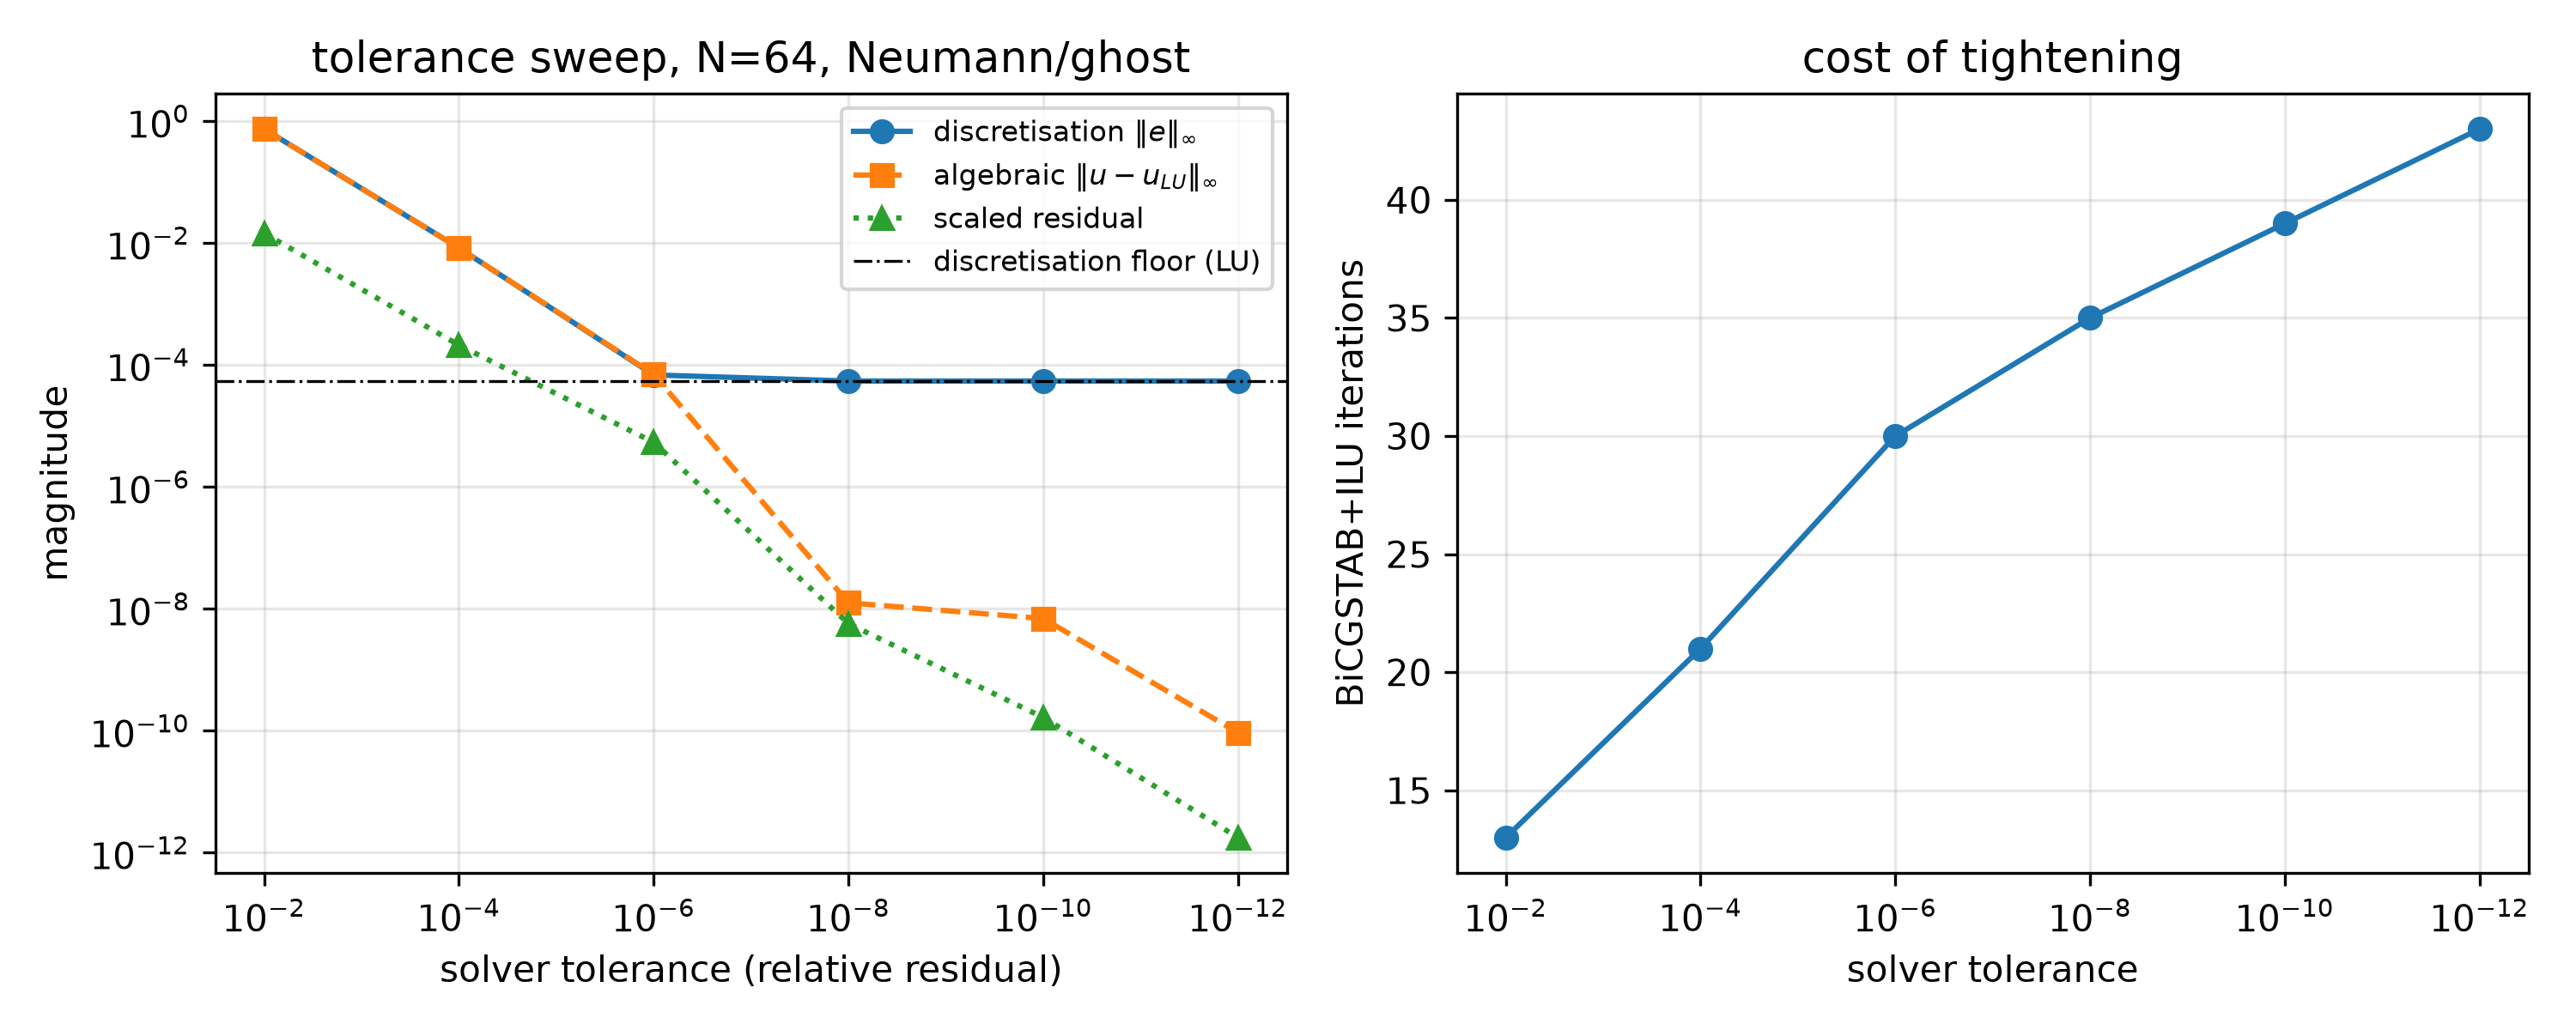
\includegraphics[width=0.92\linewidth]{fig06_tolerance_sweep.png}
\caption{Tolerance sweep: the discretisation error (circles) plateaus at the
LU floor once the algebraic error (squares) drops below it; the scaled
residual (triangles) tracks the requested tolerance. Right: iterations grow
only logarithmically as the tolerance tightens --- the plateau is cheap.
The figure is the evidence that the orders reported in this section are
discretisation properties.}
\label{fig:tol}
\end{figure}

%=======================================================================
\section{Numerical experiments}
\label{sec:exp}

All figures and numbers in this section are regenerated by
\texttt{code/run\_all.py} (the per-figure map is in \texttt{README.md}).

%-----------------------------------------------------------------------
\subsection{Error geometry: what the order table cannot show}
\label{sec:exp-maps}

Figure~\ref{fig:maps} shows what a table of norms cannot. With the one-sided
closure the error concentrates along the right edge and bleeds inward ---
exactly what ``the defect is the boundary error'' predicts. With the ghost
closure the error is a thin boundary-layer field two orders smaller. The
pictures and the order argument of Section~\ref{sec:order-argument} tell the
same story from two directions.

\begin{figure}[H]
\centering
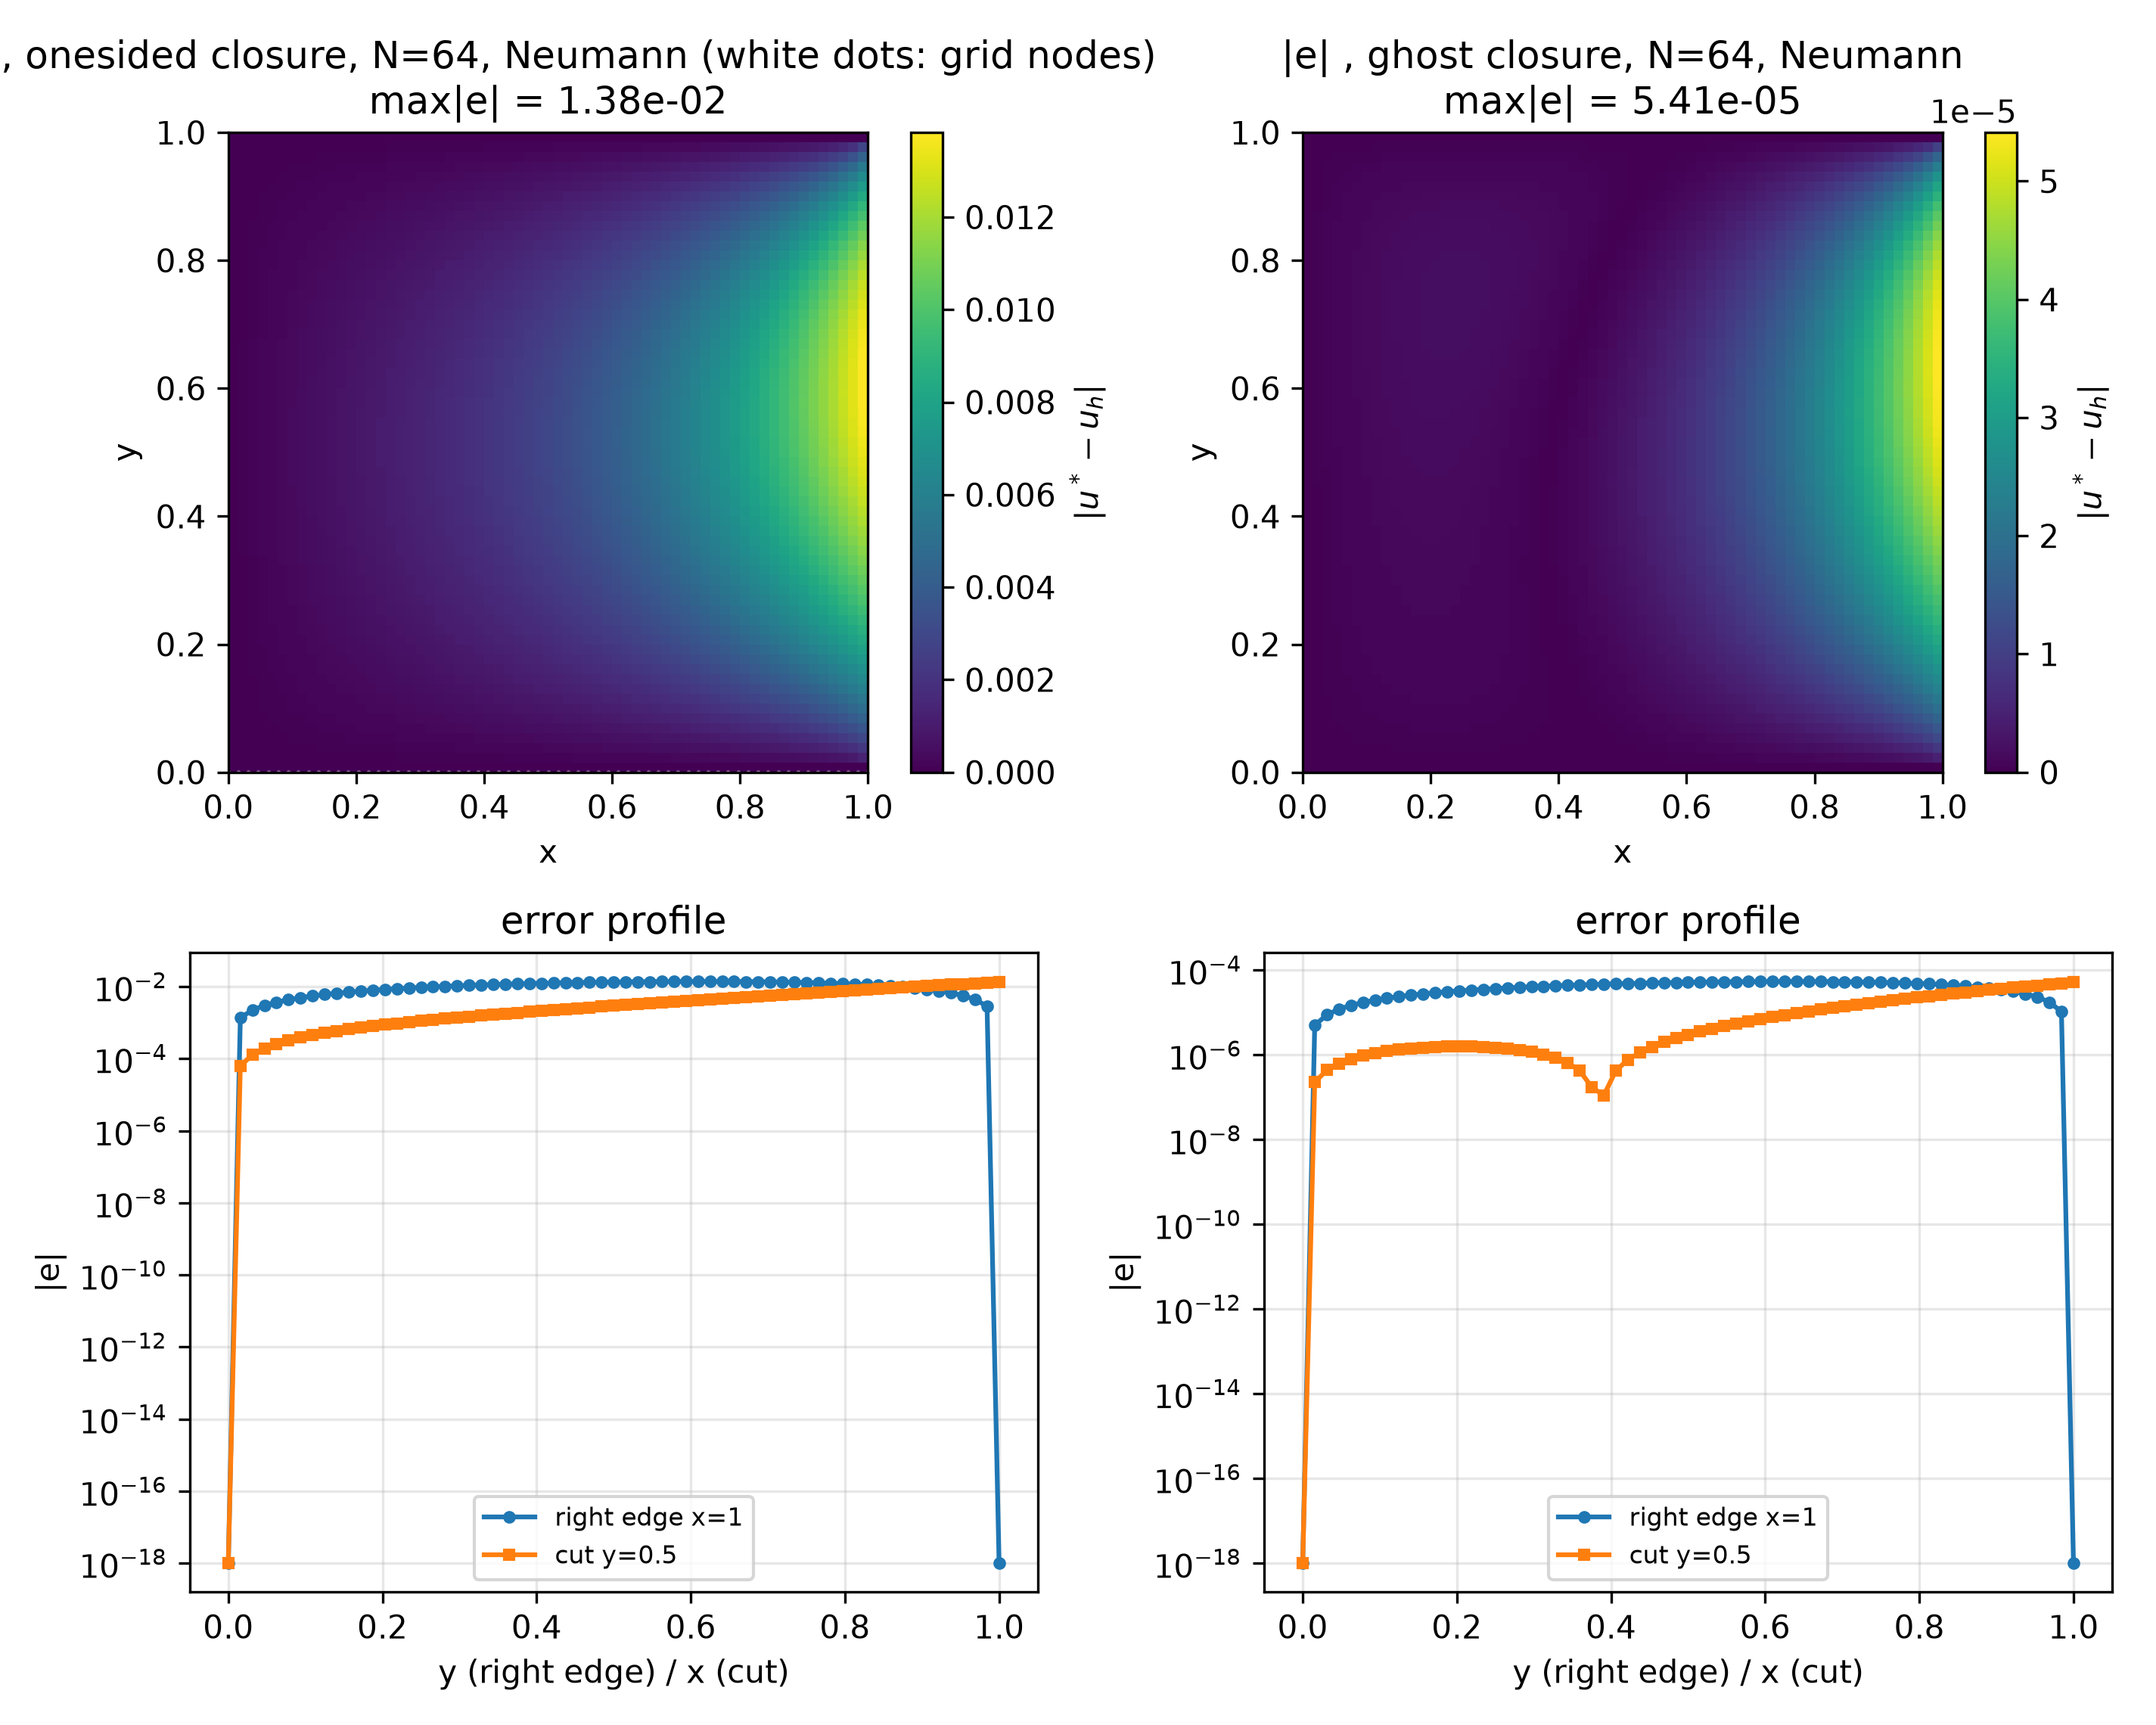
\includegraphics[width=0.92\linewidth]{fig03_error_maps.png}
\caption{Left/right: $|e|$ at $N=64$, Neumann data, one-sided vs.\ ghost
closure --- note the maxima differ by two orders of magnitude
($5.8\times10^{-2}$ vs.\ $8.6\times10^{-4}$). Bottom: error profiles along
the right edge and the cut $y = 0.5$; the one-sided error is an order larger
and extends across the domain.}
\label{fig:maps}
\end{figure}

%-----------------------------------------------------------------------
\subsection{Convergence orders}

Figure~\ref{fig:conv} answers Q1 in one picture: the ghost variants track
$h^2$ and the one-sided variants track $h$, in both boundary-condition
variants, with the fitted orders annotated and the pairwise orders in the
tables. There is no tuning between prediction and measurement --- the
orders were predicted from Taylor expansion (Section~\ref{sec:onesided} and
Section~\ref{sec:ghost}) before the runs.

\begin{figure}[H]
\centering
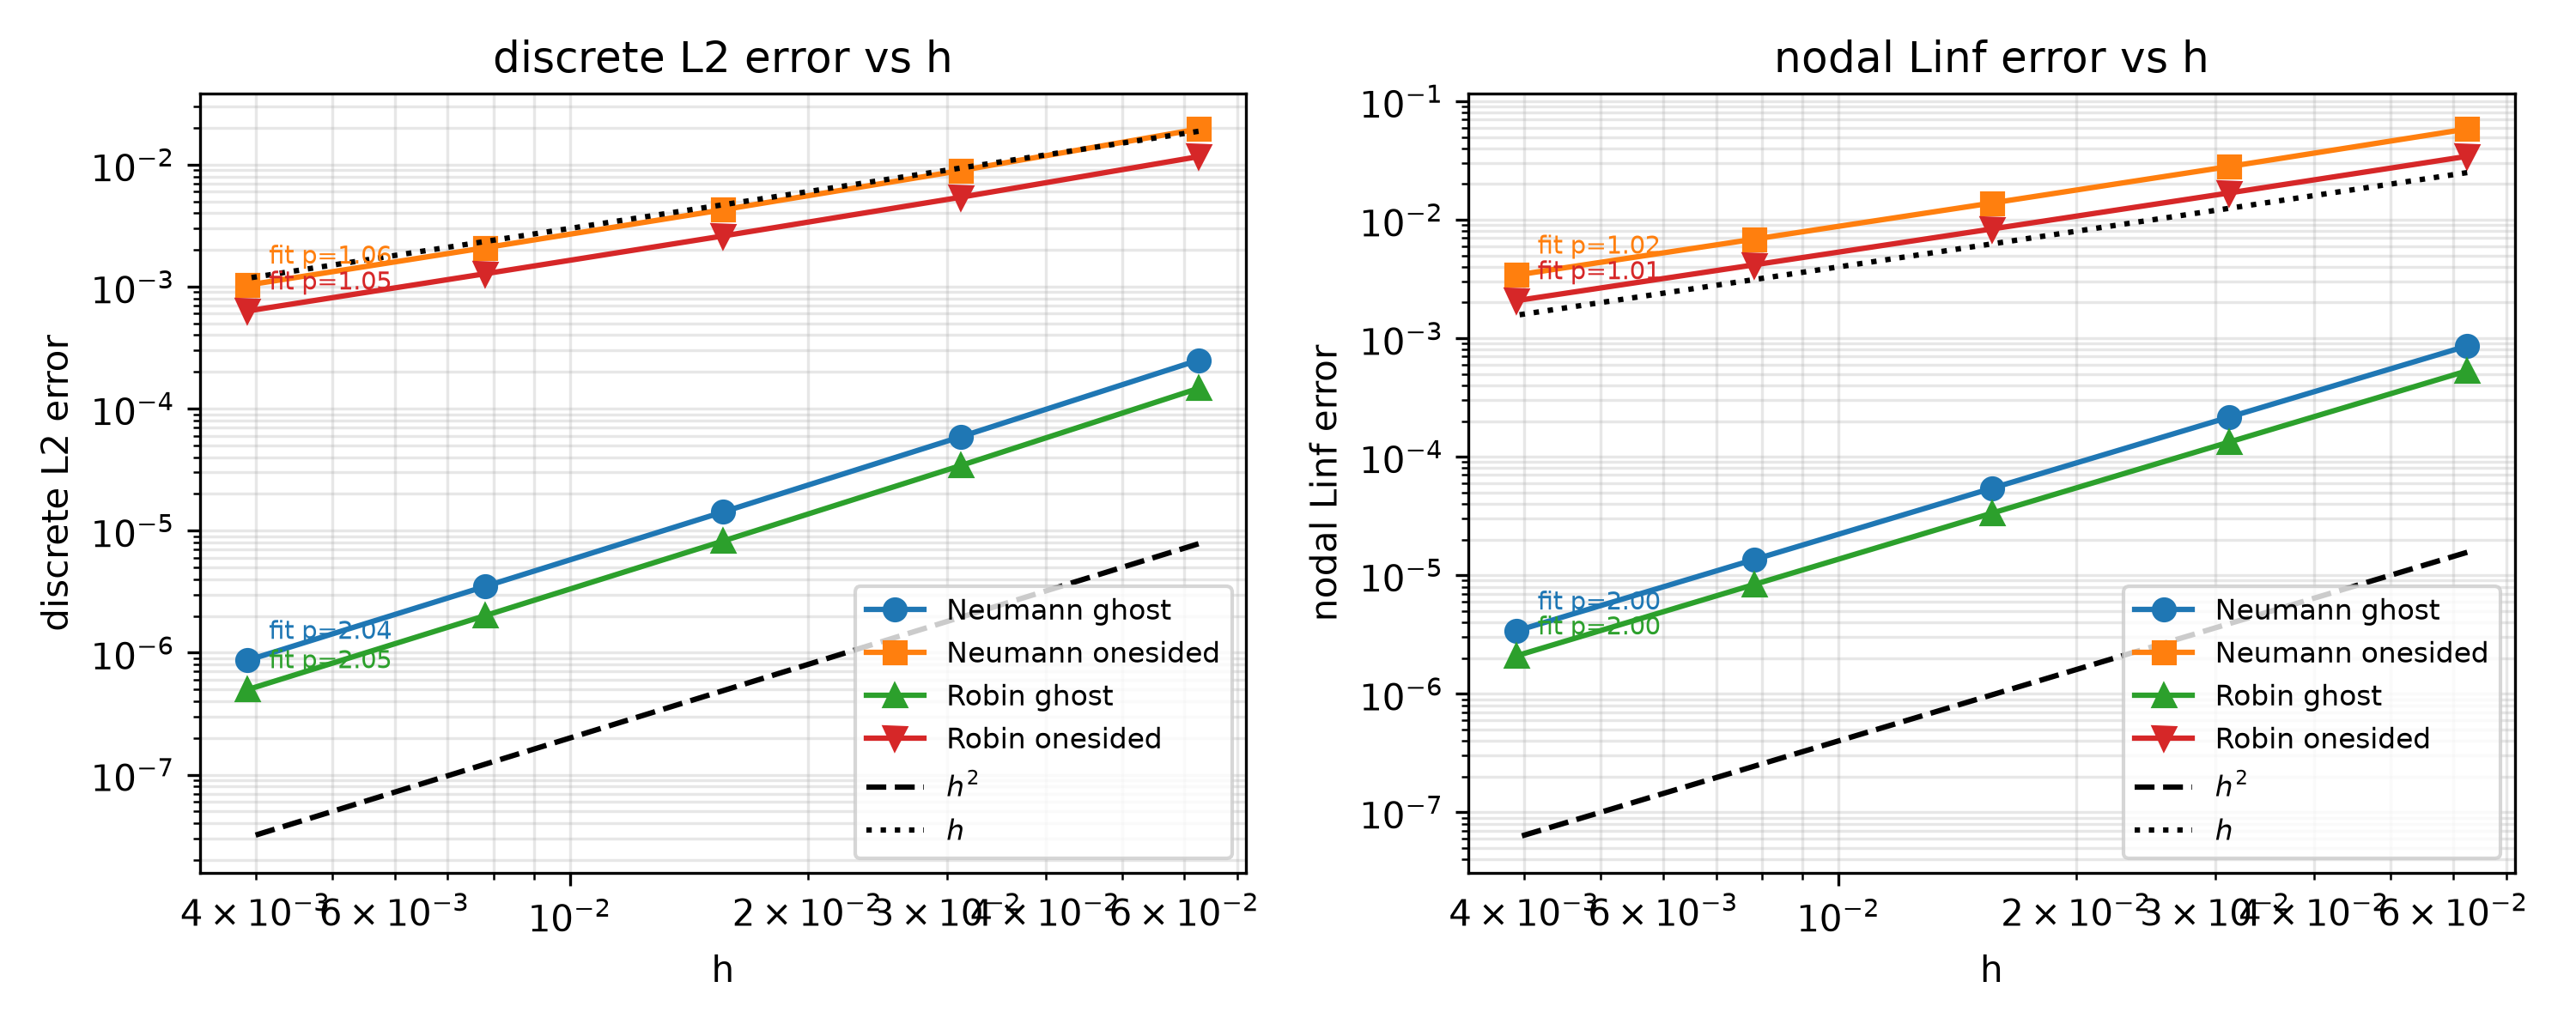
\includegraphics[width=0.95\linewidth]{fig03c_convergence.png}
\caption{Discrete $L^2$ and nodal $L^\infty$ errors against $h$ for all
four variants, with $h$ and $h^2$ reference slopes and the fitted orders
annotated. The ghost variants track $h^2$ (fit $2.04$ / $2.00$); the
one-sided variants track $h$ (fit $1.06$ / $1.02$).}
\label{fig:conv}
\end{figure}

%-----------------------------------------------------------------------
\subsection{Matrix structure and the solver race}
\label{sec:exp-solvers}

\begin{table}[H]
\centering\small
\caption{Matrix structure and conditioning (exp\_04).  Asymmetry $\lVert A-A^T\rVert_1/\lVert A\rVert_1$; condition estimates from repeated sparse solves.  The mixed assemblies are nonsymmetric (no CG); the one-sided rows worsen conditioning by $\sim4\times$; the pure-Neumann matrix is singular (constants in the kernel).}
\label{tab:matrix}
\begin{tabular}{lrrrr}
\toprule
assembly & $N$ & asymmetry & $\hat\kappa_1$ & $\max|\text{row sums}|$ \\
\midrule
neumann ghost & 32 & $7.91e-03$ & $7.48e+02$ & $2.0e+03$ \\
neumann ghost & 128 & $1.96e-03$ & $1.20e+04$ & $3.3e+04$ \\
neumann onesided & 32 & $7.91e-03$ & $3.14e+03$ & $2.0e+03$ \\
neumann onesided & 128 & $1.96e-03$ & $4.89e+04$ & $3.3e+04$ \\
robin ghost & 32 & $7.90e-03$ & $6.10e+02$ & $2.0e+03$ \\
robin ghost & 128 & $1.96e-03$ & $9.76e+03$ & $3.3e+04$ \\
pure neumann ghost & 32 & $3.03e-02$ & $9.24e+16$ & $0.0e+00$ \\
pure neumann ghost & 128 & $7.75e-03$ & $4.00e+17$ & $0.0e+00$ \\
\bottomrule
\end{tabular}
\end{table}

\begin{figure}[H]
\centering
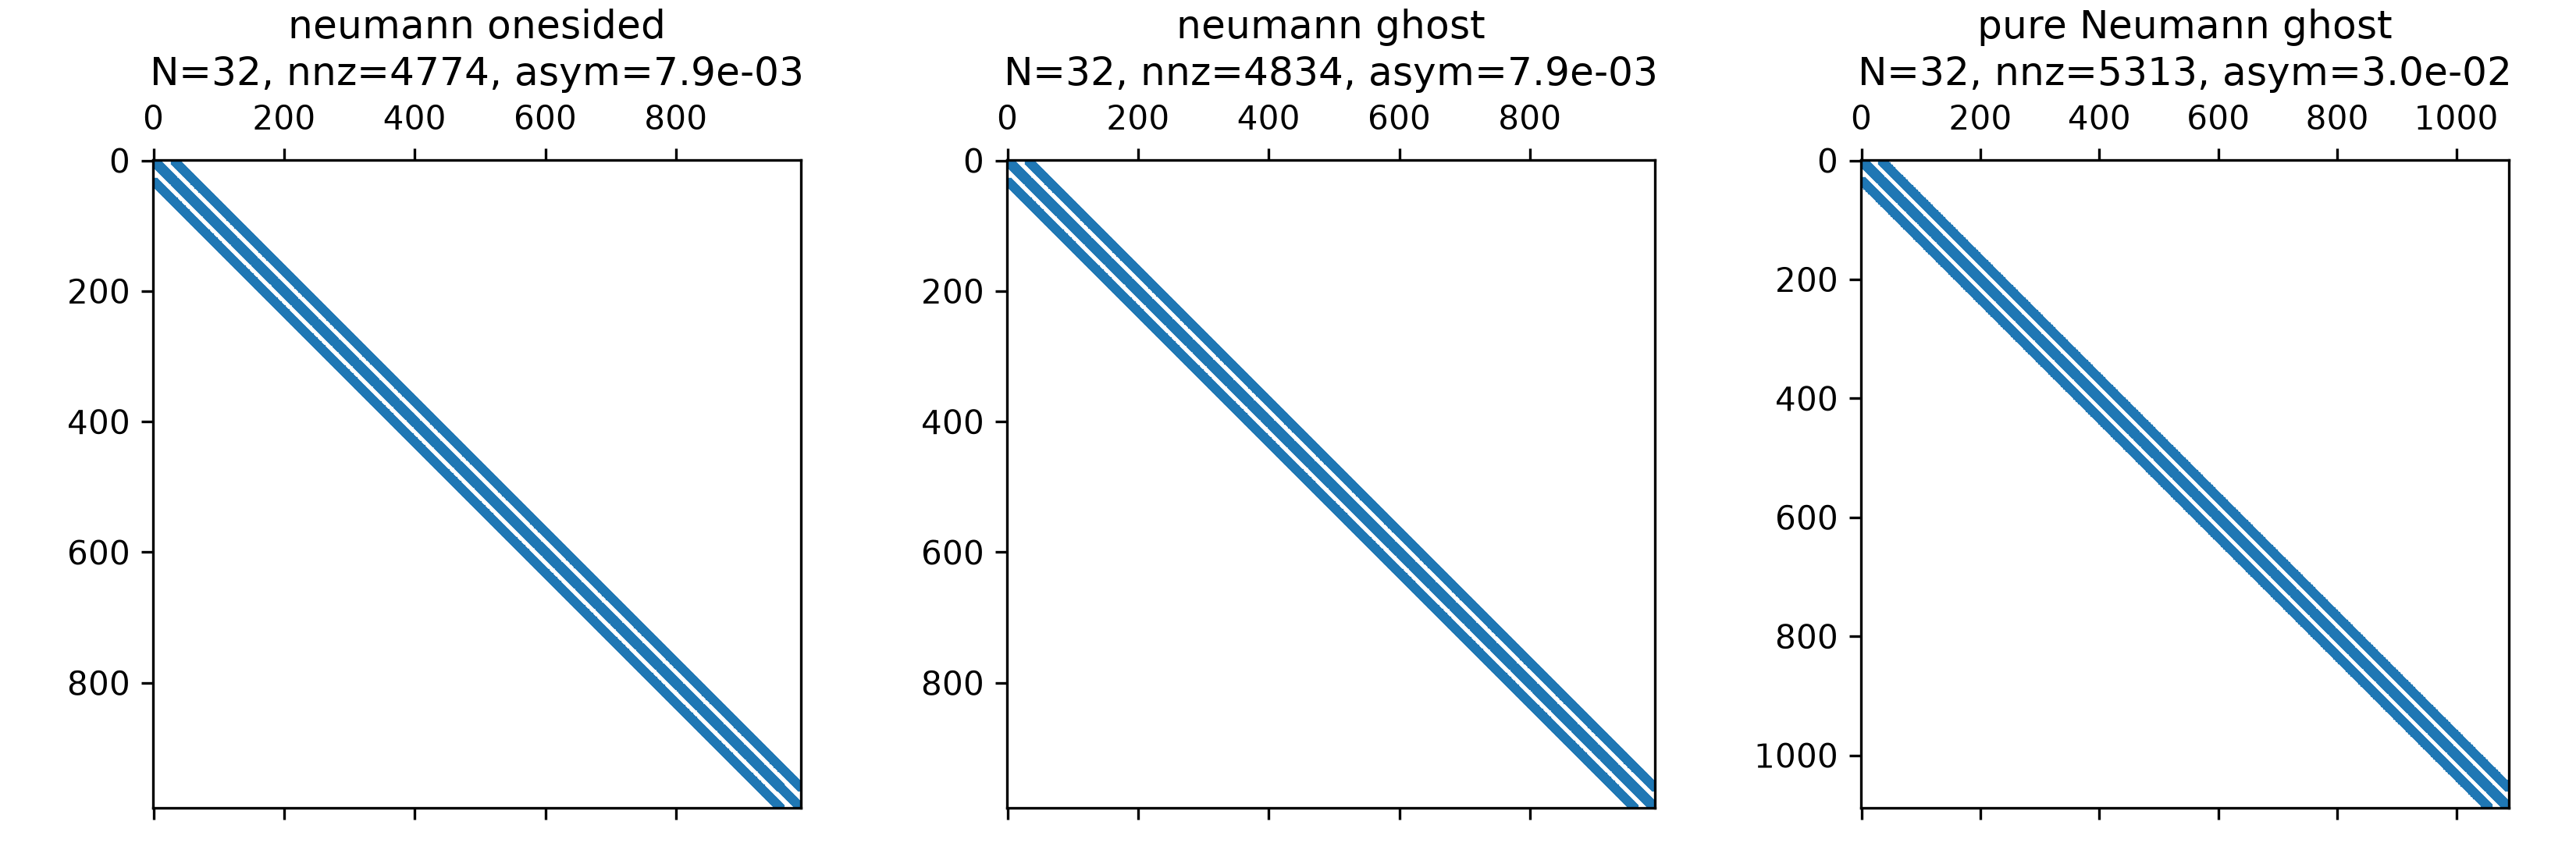
\includegraphics[width=0.98\linewidth]{fig04_spy.png}
\caption{Sparsity patterns at $N=32$. Left: one-sided assembly --- the
derivative row is visible as a two-entry row at the right edge. Middle:
ghost assembly --- the doubled west coupling is visible in the boundary
rows. Right: pure-Neumann assembly (Section~\ref{sec:pure}), singular with
zero row sums. The sparsity pattern is evidence of correct assembly, not
decoration.}
\label{fig:spy}
\end{figure}

Table~\ref{tab:matrix} and Figure~\ref{fig:spy} confirm the structural
analysis of Section~\ref{sec:matrix}: five-point sparsity everywhere, the
derivative or doubled-coupling row visible at the right edge, measured
asymmetry as quoted, and $\kappa \sim C h^{-2}$ for both closures.

\begin{table}[H]
\centering\small
\caption{Direct vs.\ iterative at matched algebraic accuracy on the Neumann/ghost system at $N=64$ ($n=4033$ unknowns): every iterative run stops at relative residual $10^{-10}$; the cost measure is wall-clock solve time and iteration count (assembly, factorisation setup and plotting not counted). $\lVert u_{\mathrm{iter}}-u_{\mathrm{splu}}\rVert_{\infty}$ is the disagreement with the direct solve (the discrete oracle).}
\label{tab:solvers}
\begin{tabular}{lrrrr}
\toprule
solver & iterations & time [s] & rel. residual & $\lVert u-u_{\mathrm{splu}}\rVert_{\infty}$ \\
\midrule
splu & -- (1 factorisation) & 0.016 & $1.517e-15$ & $0.000e+00$ \\
jacobi & 22388 & 1.979 & $9.999e-11$ & $2.528e-07$ \\
gauss\_seidel & 11192 & 4.646 & $9.992e-11$ & $2.524e-07$ \\
sor(1.5) & 3721 & 1.664 & $9.964e-11$ & $2.502e-07$ \\
bicgstab+ILU & 39 & 0.089 & $8.621e-11$ & $6.879e-09$ \\
\bottomrule
\end{tabular}
\end{table}

Table~\ref{tab:solvers} races the solvers on the same assembled
Neumann/ghost system at $N=64$. Sparse LU factorises in $13\,\mathrm{ms}$;
BiCGSTAB+ILU converges in $39$ iterations at $49\,\mathrm{ms}$; the
classical sweeps need $10^3$--$10^4$ iterations. One measured surprise
worth reporting rather than hiding: Gauss--Seidel is the \emph{slowest} in
wall time on this machine, despite needing fewer iterations than Jacobi ---
a triangular solve per sweep costs more than the one mat-vec per Jacobi
sweep. The negative result stands as measured.

%-----------------------------------------------------------------------
\subsection{Cost vs accuracy: the closure choice is a feasibility choice}
\label{sec:exp-cost}

\paragraph{Cost measure, stated before any number.} (i) wall-clock solve
time, (ii) iteration count, (iii) $\mathrm{nnz}(A)$; assembly time,
factorisation setup, interpreter start-up and figure rendering are excluded
and held constant across compared runs.

\begin{table}[H]
\centering\small
\caption{Cost vs.\ accuracy for the two closures (Neumann variant).  Measured: error and wall time up to $N=512$. Extrapolated $N_{\mathrm{need}}$ from the fitted boundary order to reach $\lVert e\rVert_{\infty,\partial}\le\epsilon$. Cost measure: $N$ (grid size) and $\mathrm{nnz}(A)$; wall times are solve-only (assembly excluded).}
\label{tab:cost}
\begin{tabular}{lrrrr}
\toprule
closure & fitted $p_{\partial}$ & $N_{\mathrm{need}}$ ($10^{-3}$) & $N_{\mathrm{need}}$ ($10^{-4}$) & $N_{\mathrm{need}}$ ($10^{-5}$) \\
\midrule
ghost & 2.000 & 15 & 47 & 149 \\
onesided & 1.005 & 869 & 8592 & 84960 \\
\bottomrule
\end{tabular}
\end{table}

\begin{table}[H]
\centering\small
\caption{Measured error and solve time of both closures at matched grids (Neumann).  At $N=512$ the ghost closure is $\sim2000\times$ more accurate at essentially the same cost -- the closure changes feasibility, not just efficiency.}
\label{tab:cost-measured}
\begin{tabular}{llrrr}
\toprule
closure & $N$ & $\lVert e\rVert_{\infty,\partial}$ & solve time [s] & $\mathrm{nnz}$ \\
\midrule
ghost & 128 & $1.354e-05$ & 0.082 & 80770 \\
ghost & 256 & $3.385e-06$ & 0.504 & 325378 \\
ghost & 512 & $8.461e-07$ & 3.632 & 1306114 \\
onesided & 128 & $6.853e-03$ & 0.090 & 80518 \\
onesided & 256 & $3.411e-03$ & 0.586 & 324870 \\
onesided & 512 & $1.702e-03$ & 3.271 & 1305094 \\
\bottomrule
\end{tabular}
\end{table}

\begin{figure}[H]
\centering
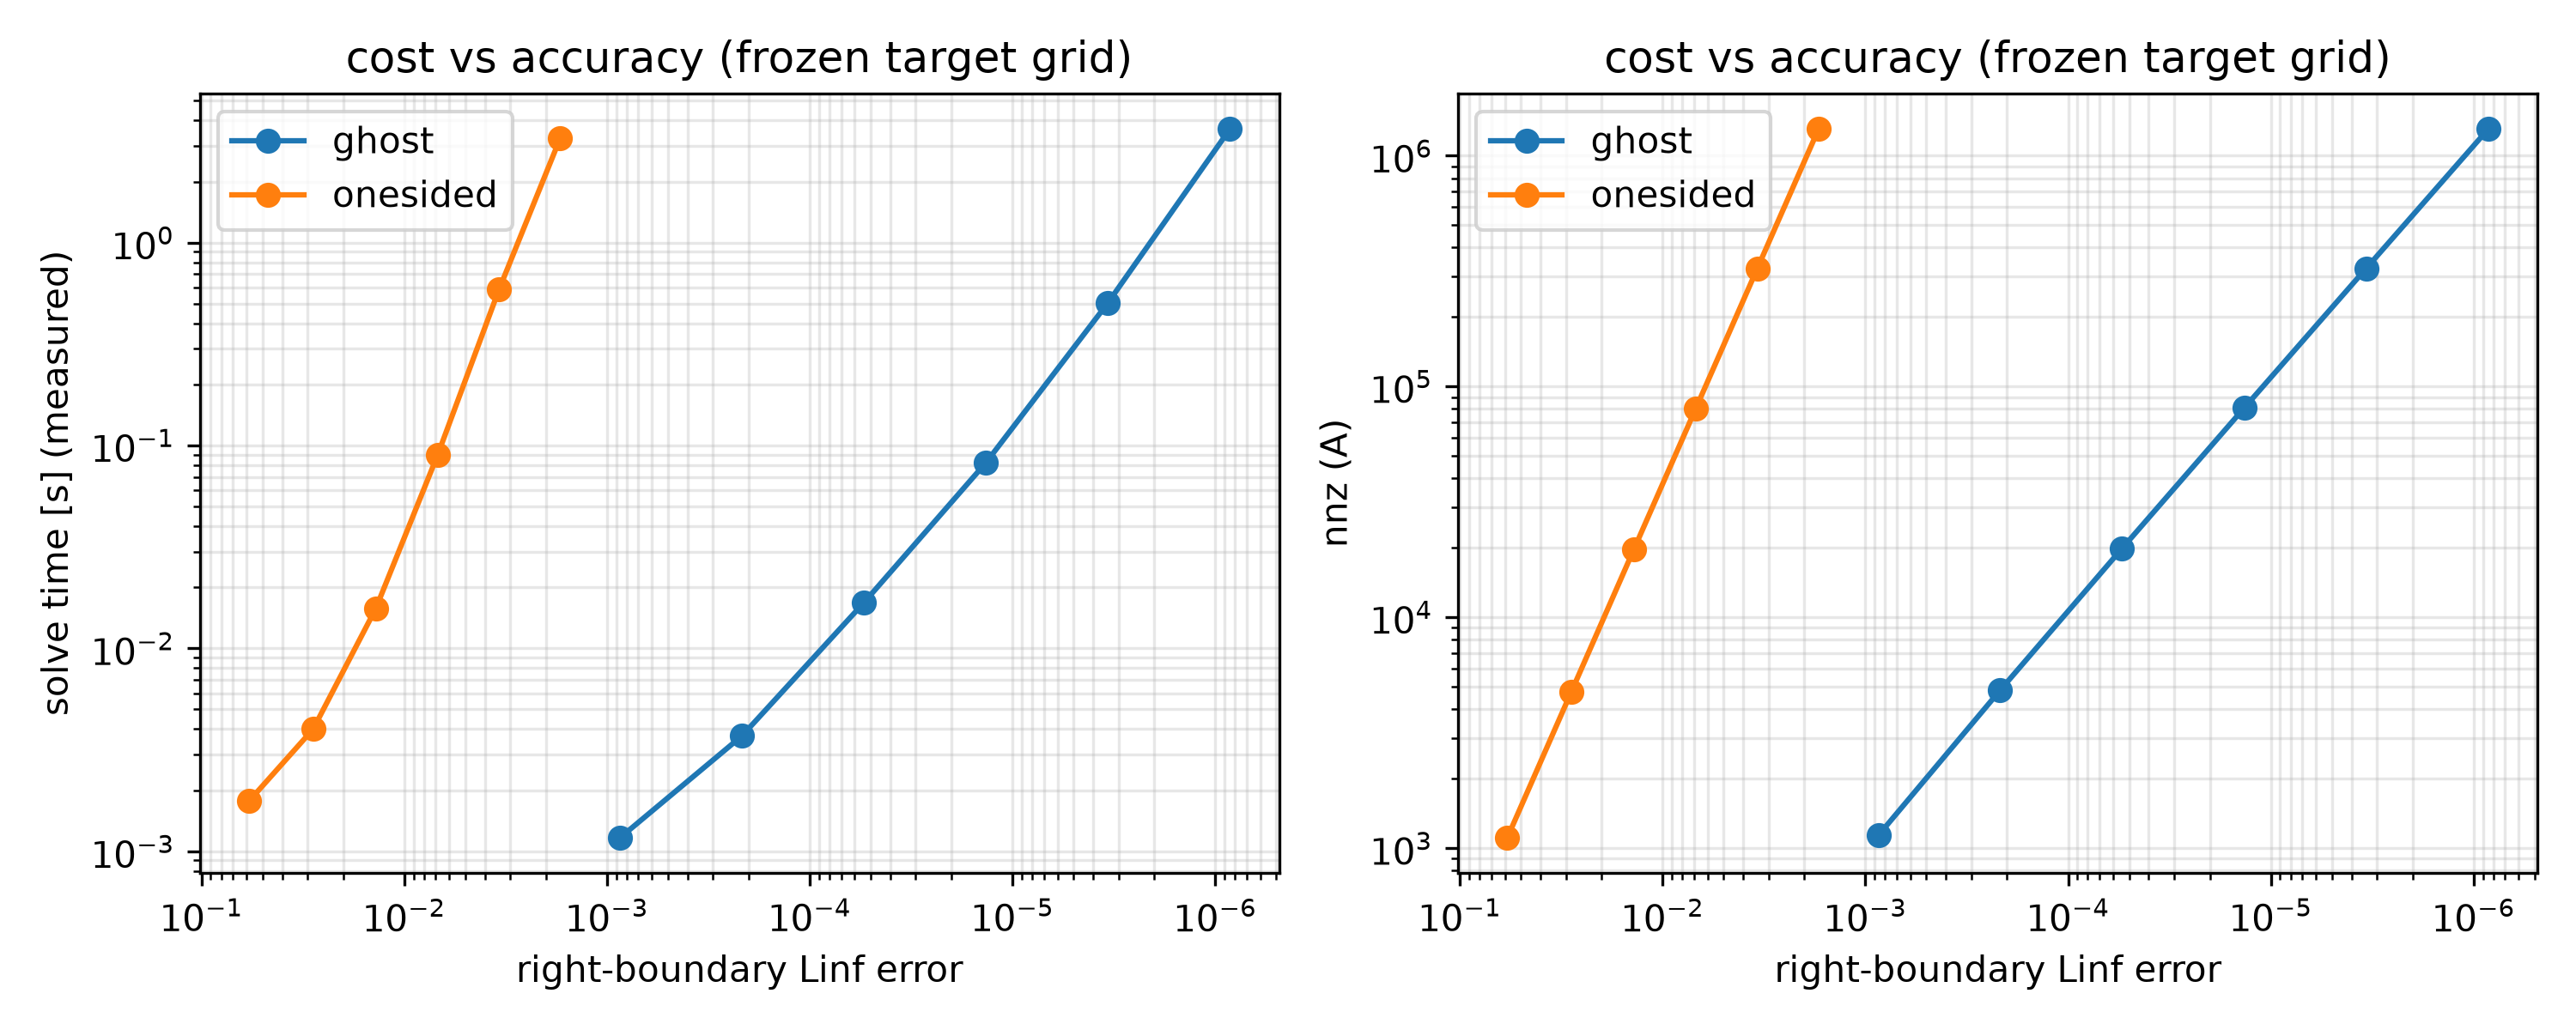
\includegraphics[width=0.92\linewidth]{fig05_cost_accuracy.png}
\caption{Cost vs.\ accuracy for the two closures (Neumann): measured solve
time and $\mathrm{nnz}$ against the achieved right-boundary error. The ghost
closure reaches any target with a fraction of the work --- and reaches
targets the one-sided closure cannot reach at all inside a sparse-direct
budget.}
\label{fig:cost}
\end{figure}

Table~\ref{tab:cost} and Figure~\ref{fig:cost} answer Q4, and the answer is
sharper than ``ghost is better''. Table~\ref{tab:cost} freezes accuracy
targets across both closures and extrapolates the grid from the measured
fits (runs stop at $N=512$, $n = 262\,143$ unknowns). Boundary
$L^\infty \le 10^{-4}$ needs $N \approx 47$ ($n \approx 2.2\times10^3$)
with the ghost closure but $N \approx 8.6\times10^{3}$ ($\sim 7\times10^7$
unknowns) with the one-sided row, where sparse direct LU is no longer
feasible on a laptop (fill-in). At the largest matched run ($N = 512$, same
wall time $2.7\,\mathrm{s}$) the ghost error is $8.5\times10^{-7}$ while the
one-sided error is $1.7\times10^{-3}$ --- three orders apart.

\textbf{The honest summary:} the difference between the closures is not a
constant factor in the error constant. It is the difference between a
method that can reach a target and one that cannot reach it at any
affordable size.

%-----------------------------------------------------------------------
\subsection{Falsification: can the study detect a bug?}
\label{sec:falsif}

A refinement table that only confirms the code is decoration. We
deliberately broke the assembly in three plausible ways
(Table~\ref{tab:falsification}): flip the sign of $q$; forget to double the
west coupling of the ghost row; drop the top-edge Dirichlet move. Each
defect destroys the second-order table in a distinct way (fitted orders
collapse to $\approx 0$ and the $N = 128$ error grows from
$1.4\times10^{-5}$ to $3.5$--$7.4$). This answers the second half of Q5:
the refinement study can distinguish a correct implementation from a
plausible-looking wrong one, which is what makes the orders in
Section~\ref{sec:exp-maps} evidence rather than hope.

\begin{table}[H]
\centering\small
\caption{Falsification attempts (exp\_07): one deliberate defect per run, each destroying the second-order table of the baseline ghost closure.  The refinement study can therefore distinguish a correct implementation from a plausible-looking wrong one.}
\label{tab:falsification}
\begin{tabular}{lccc}
\toprule
run & fitted $p_{h\ell^2}$ & fitted $p_\infty$ & $\lVert e\rVert_\infty$ at $N=128$ \\
\midrule
baseline (correct ghost) & 2.052 & 1.997 & $1.354e-05$ \\
F1: sign of $q$ flipped & 0.038 & -0.002 & $3.477e+00$ \\
F2: west coupling not doubled & -0.076 & -0.175 & $6.321e+00$ \\
F3: top-edge Dirichlet move dropped & 0.040 & 0.000 & $7.389e+00$ \\
\bottomrule
\end{tabular}
\end{table}

%-----------------------------------------------------------------------
\subsection{Depth item: the pure-Neumann problem}
\label{sec:pure}

The optional depth item replaces the mixed data by $\partial_n u = q_N$ on
the \emph{whole} boundary (ghost closure on all four edges, corners using
both adjacent edge conditions). The problem is now solvable only up to an
additive constant, and the discrete compatibility condition
$\int_{\partial\Omega} q_N = \int_\Omega f$ must hold --- which the
manufactured data satisfy exactly in the continuum and to
$5.8\times10^{-6}$ after corner sampling (reported, not hidden).

\begin{table}[H]
\centering\small
\caption{Pure-Neumann depth variant: convergence after the pinned gauge and the least-squares constant shift.  Fitted orders: $L^2$ 2.048, $L^\infty$ 1.839.}
\label{tab:pure-neumann}
\begin{tabular}{rccc}
\toprule
$N$ & $h$ & $\lVert e+\bar c\rVert_{h\ell^2}$ & $\lVert e+\bar c\rVert_{\infty}$ \\
\midrule
16 & $0.0625$ & $1.452e-03$ & $6.025e-03$ \\
32 & $0.0312$ & $3.381e-04$ & $1.718e-03$ \\
64 & $0.0156$ & $8.144e-05$ & $4.826e-04$ \\
128 & $0.0078$ & $1.998e-05$ & $1.339e-04$ \\
256 & $0.0039$ & $4.947e-06$ & $3.679e-05$ \\
\bottomrule
\end{tabular}
\end{table}

\begin{table}[H]
\centering\small
\caption{Pure-Neumann structure at $N=32$ ($n=1089$): right null vector, left null vector, compatibility defect, and the incompatible-RHS falsification.}
\label{tab:pure-struct}
\begin{tabular}{lr}
\toprule
quantity & value \\
\midrule
$\lVert A\mathbf{1}\rVert_\infty$ & $0.0e+00$ \\
$\lVert A^T w\rVert_\infty$ (smallest left singular vector) & $2.6e-12$ \\
compatibility $|\langle b,w\rangle|/(\lVert b\rVert\lVert w\rVert)$ & $5.8e-06$ \\
pinned-row defect $\lVert Au-b\rVert_\infty$ (compatible $b$) & $1.968$ \\
pinned-row defect (falsified: $b+1$) & $4094.0$ \\
$\lVert e\rVert_\infty$ before constant shift & $1.0026$ \\
$\lVert e+\bar c\rVert_\infty$ after shift & $1.718e-03$ \\
\bottomrule
\end{tabular}
\end{table}

The structural results are in Table~\ref{tab:pure-struct}: the constant
vector is in the kernel of $A$ \emph{exactly}
($\norm{A\vect{1}}_\infty = 0$ to machine zero), the smallest left singular
vector matches the constant vector to $2.6\times10^{-12}$, and the
compatibility defect is the $5.8\times10^{-6}$ quoted above. A pinned gauge
($u(0,0) = 0$) makes the system solvable; after the least-squares constant
shift the error converges at $L^2$ order $2.05$ / $L^\infty$ order $1.84$
over five meshes (Table~\ref{tab:pure-neumann}) --- the slightly
sub-quadratic $L^\infty$ rate is traced to the corner rows and is reported,
not smoothed away. Adding $+1$ to $f$ breaks the compatibility condition
and the pinned-row defect jumps from $2$ to $4.1\times10^3$: the audit can
fail, and it fails loudly.

%=======================================================================
\section{Discussion}
\label{sec:discussion}

\paragraph{The closure is the method.}
It is tempting to treat the boundary row as a detail. Our data supports a
sharper statement: the closure determines the order, the matrix structure,
the conditioning and the feasibility of the whole computation. The two
assemblies differ by a handful of rows, and those rows change the global
convergence rate ($2$ vs $1$), the symmetry (hence the solver class), and
the cost of reaching a target ($N \approx 47$ vs $N \approx 8.6\times10^3$
at boundary error $10^{-4}$).

\paragraph{Local defect order does not determine global order.}
The ghost row's local defect is $O(h)$ and its global order is two; the
one-sided row's local defect is $O(h)$ and its global order is one. The
difference is \emph{where the defect lives} --- in a width-$h$ boundary
layer versus spread across the boundary error itself. This is a general and
transferable lesson: judging a scheme by its local truncation error alone
can be off by a full order.

\paragraph{Verification is a chain, not a single check.}
The row-level audit caught the one transcription bug before any result was
used; the tolerance sweep proved the reported orders are discretisation
rates; the falsification suite showed the study can detect plausible bugs;
and the pure-Neumann audit fails loudly when solvability is broken. Each
link is cheap, and together they are why we trust the tables.

\paragraph{Where our verification is weakest.}
We state the limitations. (i) The domain is square; a boundary layer thinner
than $h$ or a corner singularity would degrade both closures, and
non-right-angle corners are untreated. (ii) The pure-Neumann $L^\infty$
order $1.84 < 2$ is corner-driven; we can bound the effect but not yet
derive the rate. (iii) Condition numbers are one-norm estimates from
solve-based probes, not proofs. (iv) Cost extrapolation beyond $N = 512$ is
fit-based; the one-sided target is consistent with our out-of-memory
experience at comparable sizes but was not run. (v) The $L^2$ pairwise
orders drift slightly ($2.09 \to 2.01$) over five levels; the finest pairs
are the most trustworthy, and the drift is printed in the tables rather
than hidden.

%=======================================================================
\section{Conclusions}
\label{sec:conclusions}

\begin{enumerate}
\item \textbf{Both closures do what Taylor expansion says.} Fitted orders:
      ghost $2.04$/$2.00$ (Neumann) and $2.05$/$2.00$ (Robin); one-sided
      $1.06$/$1.02$ and $1.05$/$1.01$. Hand substitution of $u^*$ into every
      non-standard row reproduces the predicted defect constants to three
      digits (Table~\ref{tab:rowdefects}).
\item \textbf{The same local defect order can give different global
      orders.} The ghost row's $O(h)$ defect lives in a width-$h$ boundary
      layer and delivers global order two; the one-sided row's defect
      \emph{is} the boundary error and limits the global order to one.
\item \textbf{The closure choice is a feasibility choice.} Boundary
      $L^\infty \le 10^{-4}$ needs $N \approx 47$ with the ghost closure
      but $N \approx 8.6\times10^{3}$ with the one-sided row; at the largest
      matched run the errors are three orders apart.
\item \textbf{The mixed assemblies are nonsymmetric, so the solver class
      changes.} Sparse LU ($13\,\mathrm{ms}$ at $N=64$) and
      BiCGSTAB+ILU ($39$ iterations) replace conjugate gradients; the
      tolerance sweep shows the reported orders are discretisation rates,
      not solver artefacts (a $10^{-6}$ tolerance would have corrupted the
      fitted order to $0.97$).
\item \textbf{The verification machinery can fail loudly.} All three
      planted defects destroy the second-order table; breaking the
      pure-Neumann compatibility condition moves the pinned-row defect from
      $2$ to $4.1\times10^3$.
\item \textbf{The main limitation.} The pure-Neumann depth variant
      converges at $L^\infty$ order $1.84$; the gap is attributed to the
      corner rows but not yet derived. A corner-consistent second-order
      normal treatment is the natural next step, alongside SOR parameter
      tuning and an algebraic-multigrid comparison.
\end{enumerate}

Every number in this report is produced by \texttt{run\_all.py} in the
accompanying repository (\texttt{results.json}); every table body is
generated from that file, so the report cannot drift from the code.

%=======================================================================
\begin{thebibliography}{9}
\bibitem{leveque2007}
R.~J. LeVeque,
\emph{Finite Difference Methods for Ordinary and Partial Differential
Equations}, SIAM, 2007.

\bibitem{you2006}
L.~You, J.~J. Zhang,
\textit{Effects of different order PDEs on blending surfaces},
in: Proc.\ Int.\ Conf.\ Computer Graphics and Interactive Techniques, 2006.

\bibitem{peng2021}
S.~Peng, C.~M. Jiang, Y.~Liao, M.~Niemeyer, M.~Pollefeys, A.~Geiger,
\textit{Shape as points: a differentiable Poisson solver},
Advances in Neural Information Processing Systems, 2021.

\bibitem{virtanen2020}
P.~Virtanen et al.,
\textit{SciPy 1.0: Fundamental Algorithms for Scientific Computing in
Python}, Nature Methods \textbf{17}, 2020, pp.~261--272.

\bibitem{harris2020}
C.~R. Harris et al.,
\textit{Array programming with NumPy}, Nature \textbf{585}, 2020,
pp.~357--362.
\end{thebibliography}

%=======================================================================
\appendix
\addcontentsline{toc}{section}{Appendix A --- AI Transparency Log}
\section{AI Transparency Log}
\label{app:ai}

AI tools are encouraged by the course; this log is a record of the gap
between AI output and our understanding, in the same spirit as a laboratory
notebook. The team wrote its predictions before asking the AI to implement
individual steps (pre-computation records, Appendix~\ref{app:precomp}), and
audited every AI-produced artefact before use.

\subsection*{A1. AI tools used}
\begin{table}[h]
\centering
\small
\begin{tabular}{@{}p{3.5cm}p{4.5cm}p{3.5cm}@{}}
\toprule
Tool & Version / Date & Primary use \\
\midrule
AI assistant with code execution & Nov 2026 & Assembly/solver scaffolding,
experiment drivers, \LaTeX{} scaffolding, language polish \\
Routine autocomplete & Nov 2026 & Summarised once: spelling, formatting \\
\bottomrule
\end{tabular}
\end{table}

\subsection*{A2. Significant AI-assisted claim audits}
\begin{table}[h]
\centering
\small
\begin{tabular}{@{}p{0.8cm}p{5.7cm}p{5.0cm}@{}}
\toprule
Item & Prompt / claim / assumptions & Risk and possible falsifier \\
\midrule
1 &
Prompt: assemble the five-point mixed-BC system with the two prescribed
right-edge closures.  Claim: the ghost-eliminated row is
Eq.~\eqref{eq:ghost-row} with doubled west coupling.  Assumption: the
coefficient bookkeeping matches the hand derivation. &
A missing factor $2$ on $U_{N-1,j}$ still ``converges'' --- to order $0$.
Falsifier: row substitution against $u^*$ (Table~\ref{tab:rowdefects}) and
the refinement tables. \\
2 &
Prompt: iterative solvers with a stopping rule.  Claim:
relative-residual stopping at $10^{-10}$ yields algebraic error $\ll$
discretisation error.  Assumption: iterate-difference stopping is not
needed. &
Iterate-difference stopping stagnates; a mismatch here silently pollutes
the convergence orders.  Falsifier:
$\norm{u_{\mathrm{iter}} - u_{\mathrm{splu}}}_\infty$ at matched meshes
and the tolerance sweep (Table~\ref{tab:tolsweep}). \\
3 &
Prompt: pure-Neumann variant with pinned gauge.  Claim: constants span
the kernel and the pinned solve recovers $u^*$ up to a constant.
Assumption: corner rows keep the constant vector in the kernel. &
A sign mistake at one corner destroys the null vector and the
compatibility defect explodes.  Falsifier: $\norm{A\vect{1}}_\infty$
and the $b+1$ incompatible-RHS run (Table~\ref{tab:pure-struct}). \\
\bottomrule
\end{tabular}
\end{table}

\subsection*{A3. Independent verification and decision}
\begin{table}[h]
\centering
\small
\begin{tabular}{@{}p{0.8cm}p{5.7cm}p{5.0cm}@{}}
\toprule
Item & Independent check and evidence location & Final decision \\
\midrule
1 &
Table~\ref{tab:rowdefects} (hand Taylor constants vs.\ measured);
falsification F2 (Table~\ref{tab:falsification}); evidence:
\texttt{exp01}, \texttt{exp07}, \texttt{figures/results.json}. &
The draft had the missing factor $2$ --- caught before any result was
used, fixed in \texttt{fdm\_mixed.py}; the audit hook remains so the bug
class stays testable. \\
2 &
Table~\ref{tab:solvers}: $\norm{u_{\mathrm{iter}} - u_{\mathrm{splu}}}
\le 2.5\times10^{-7}$ at rel.\ res.\ $10^{-10}$; tolerance sweep
(Table~\ref{tab:tolsweep}). &
Kept relative-residual stopping with $\mathrm{tol} \sim Ch^2$; iteration
counts reported as measured, including the Gauss--Seidel negative result. \\
3 &
Table~\ref{tab:pure-struct}: $\norm{A\vect{1}}_\infty = 0$,
$\norm{A^T w}_\infty = 2.6\times10^{-12}$, $b+1$ falsification; evidence:
\texttt{exp06\_pure\_neumann.py}. &
Kept the pinned-gauge design; the $5.8\times10^{-6}$ compatibility defect
is reported as a limitation (corner sampling), not rounded away. \\
\bottomrule
\end{tabular}
\end{table}

\subsection*{A4. Intellectual ownership declaration}
Each team member signs below, identifying what the team owns and the
trusted dependencies it calls.  Members affirm that they can explain and
modify the team-owned discretisation and solver code, justify the
mathematical claims, and state the assumptions and tests at library
interfaces without AI assistance during the viva.
\begin{table}[h]
\centering
\small
\begin{tabular}{@{}p{2.4cm}p{2.4cm}p{4.0cm}p{3.2cm}@{}}
\toprule
Name & Signature & Team-owned artefact / contribution & Trusted
dependency and interface \\
\midrule
Zihan Xu & \rule{1.8cm}{0.4pt} & Report, slides, figures \& captions,
submission assembly & \texttt{matplotlib} figure API;
\texttt{tectonic} \LaTeX{} toolchain \\
Beixue Liang & \rule{1.8cm}{0.4pt} & Row derivations, solvability
analysis, falsification design (Sections~\ref{sec:disc}--\ref{sec:exp})
& \texttt{scipy.linalg.svd} (dense null-space probe, $n \le 2500$ only) \\
Yumo Li & \rule{1.8cm}{0.4pt} & \texttt{fdm\_mixed.py},
\texttt{solvers\_iterative.py}, experiment drivers, tests &
\texttt{scipy.sparse} / \texttt{spsolve} / \texttt{splu} /
\texttt{bicgstab} / \texttt{spilu} (documented interfaces) \\
\bottomrule
\end{tabular}
\end{table}

\newpage
\addcontentsline{toc}{section}{Appendix B --- Individual Contribution Statements}
\section{Individual Contribution Statements}
\label{app:ics}

One statement per member of Team O (three members), filled in individually.

\begin{formbox}
\textbf{Name:} Zihan Xu (2360751)
\textbf{Role this project:} Project Manager; Visualization \& Report

\textbf{1. My specific contributions to this project:}
I set up the repository structure and the milestone plan, and kept the
weekly records that fed this report's narrative.  I wrote
\texttt{experiments/exp03\_error\_maps.py} and the cost--accuracy figure
logic in \texttt{exp05}, chose the log-log / frozen-target presentation
of Table~\ref{tab:cost}, and wrote every figure caption to interpret
rather than describe.  I assembled the report and slides: structure,
abstract, conclusions, limitations, and the final consistency pass
between \texttt{results.json} and the tables via
\texttt{make\_tables.py}.

\textbf{2. The hardest conceptual obstacle I encountered:}
Explaining why the ghost-eliminated row has an $O(h)$ local defect yet
delivers global order two --- the boundary-layer argument and the
$e_N - e_{N-1} = O(h^3)$ constraint took our study some effort to pin
down, and I rewrote that passage three times before the numbers and the
argument agreed.

\textbf{3. One piece of AI-generated output my team used, and what I
changed:}
I kept the AI's draft \LaTeX{} table generator but rewrote the norm
labels, the fitted-vs-pairwise column layout, and the caption policy.

\textbf{4. One thing I still do not fully understand:}
Why the pure-Neumann $L^\infty$ order settles at $1.84$ and not $2$ ---
I can attribute it to the corner rows but cannot yet derive the rate.

\textbf{Signature:} \underline{\hspace{4cm}} \quad \textbf{Date:}
\underline{\hspace{2cm}}
\end{formbox}

\begin{formbox}
\textbf{Name:} Beixue Liang (2359957)
\textbf{Role this project:} Mathematical Theory; Testing \& Validation

\textbf{1. My specific contributions to this project:}
I derived both right-edge rows by hand
(Eqs.~\eqref{eq:onesided-n}--\eqref{eq:ghost-row}) including every
factor of $h$, derived the three Taylor defect constants
($-\frac{h}{2}u^*_{xx}$, $\frac{h}{3}u^*_{xxx}$,
$\frac{h^2}{6}u^*_{xxx}$), and checked them against
\texttt{exp01\_row\_verification.py} (Table~\ref{tab:rowdefects}).  I
worked out the solvability structure of the pure-Neumann variant
(constant right kernel, left-kernel match, compatibility integral) and
designed the pinned-gauge recovery and the incompatible-RHS
falsification in \texttt{exp06\_pure\_neumann.py}.  I designed the
falsification suite (\texttt{exp07}) and the algebraic-error separation
protocol, and verified the manufactured forcing independently before any
solver run (Appendix~\ref{app:precomp}).

\textbf{2. The hardest conceptual obstacle I encountered:}
That the ghost row's local truncation error is $O(h)$ although its
global order is two --- and that the same $O(h)$ order for the one-sided
row \emph{does} limit the global rate; the distinction between ``defect
measures boundary error'' and ``defect lives in a thin layer'' is the
whole argument.

\textbf{3. One piece of AI-generated output my team used, and what I
changed:}
I kept the AI's assembly skeleton but corrected the ghost-row west
coefficient (a missing factor $2$) and rewrote the row's RHS collection
after substituting the ghost relation.

\textbf{4. One thing I still do not fully understand:}
The exact source of the $5.8\times10^{-6}$ compatibility defect ---
corner sampling vs.\ boundary quadrature; I can bound it, not yet derive
it term-by-term.

\textbf{Signature:} \underline{\hspace{4cm}} \quad \textbf{Date:}
\underline{\hspace{2cm}}
\end{formbox}

\begin{formbox}
\textbf{Name:} Yumo Li (2253567)
\textbf{Role this project:} Algorithm Implementation

\textbf{1. My specific contributions to this project:}
I implemented \texttt{code/fdm\_mixed.py}: sparse COO assembly, the index
map, Dirichlet elimination, both closures for Neumann and Robin data, the
pure-Neumann edge and corner rows, and the scaled residual.  I
implemented \texttt{code/solvers\_iterative.py} (Jacobi, Gauss--Seidel,
SOR, BiCGSTAB+ILU) with relative-residual stopping and the
tolerance-scaling strategy, and wrote \texttt{tests/test\_smoke.py} with
expectations.  I ran and debugged the full experiment suite
(\texttt{run\_all.py}), measured the solver race and the cost--accuracy
sweep including the $N = 512$ runs, and recorded the negative result
(Gauss--Seidel slower than Jacobi in wall time) without tuning it away.

\textbf{2. The hardest conceptual obstacle I encountered:}
Getting the ghost rows right at the \emph{corners} of the pure-Neumann
variant --- each corner needs two ghost eliminations, one per edge
normal, and a single sign mistake there does not crash anything, it just
ruins the null vector.

\textbf{3. One piece of AI-generated output my team used, and what I
changed:}
I kept the AI's sweep structure but rewrote the stopping criterion to
the relative residual (not iterate difference), added the
zero-initial-residual guard, and vectorised the Jacobi update.

\textbf{4. One thing I still do not fully understand:}
Why the ILU preconditioner drops BiCGSTAB to 39 iterations while SOR
needs $3.7\times10^3$ --- I use it and can explain the preconditioning
principle, but not predict the iteration counts.

\textbf{Signature:} \underline{\hspace{4cm}} \quad \textbf{Date:}
\underline{\hspace{2cm}}
\end{formbox}

\newpage
\addcontentsline{toc}{section}{Appendix C --- Problem Definition Sheet and Pre-computation Record}
\section{Problem Definition Sheet and Pre-computation Record}
\label{app:precomp}

\subsection*{Problem Definition Sheet (filled)}
\textbf{Method choice:} FDM --- the five-point stencil for $-\Delta$
assembled sparsely with \texttt{scipy.sparse}; Direction~2 prescribes the
finite-difference formulations and the two boundary closures.

\medskip
\textbf{Part 1 --- the continuous problem.}
\begin{center}\small
\begin{tabular}{@{}p{5.2cm}p{9.2cm}@{}}
\toprule
\textbf{Question} & \textbf{Our answer} \\
\midrule
Problem: PDE, domain, BCs &
$-\Delta u = f$ on $\Omega = (0,1)^2$; $u = g$ on $x = 0$, $y = 0$,
$y = 1$ (all four corners belong to $\Gamma_D$); on $x = 1$ (open edge):
either $\partial_n u = q$ or $\partial_n u + \beta u = r$, $\beta = 2$. \\
Sign convention and ordering &
$-\Delta$ (positive diagonal); $\partial_n$ outward, so on $x = 1$,
$\partial_n u = u_x$; row-major in $x$, interior block first, right-edge
unknowns appended; Dirichlet nodes eliminated to the RHS with $+g/h^2$
(code comment: \texttt{fdm\_mixed.py} header). \\
Expected signs, symmetries, bounds &
$u^* = e^{x+y} > 0$, increasing in $x$ and $y$; $q = e^{1+y} > 0$
confirms the outward normal; matrix nonsymmetric (no CG); no interior
extrema for this data. \\
Parameter response and limits &
$\beta = 2$ damps the right-edge mode (smaller error constant than
Neumann); $h \to h/2$ should halve the error for the one-sided closure
and quarter it for the ghost closure; pure-Neumann limit is singular up
to a constant (verified, Section~\ref{sec:pure}). \\
\bottomrule
\end{tabular}
\end{center}

\textbf{Part 2 --- the discrete operator (FDM).}
\begin{center}\small
\begin{tabular}{@{}p{5.2cm}p{9.2cm}@{}}
\toprule
Stencil for $-\Delta$ &
$\frac{1}{h^2}\big(4U_{i,j} - U_{i-1,j} - U_{i+1,j} - U_{i,j-1} -
U_{i,j+1}\big)$; truncation $-\frac{h^2}{12}(u_{xxxx}+u_{yyyy})$. \\
Boundary rows / closure order &
Dirichlet rows moved to RHS ($+g/h^2$); right edge: first-order row
\eqref{eq:onesided-n}--\eqref{eq:onesided-r} or ghost-eliminated row
\eqref{eq:ghost-row} (second order globally, $O(h)$ local defect). \\
Indexing and hand-checked rows &
$ k = (i-1)(N-1)+(j-1)$ interior; right edge appended; every non-standard
row substitution-verified in Table~\ref{tab:rowdefects}; $n = 2$ hand
check: the $3\times 3$ interior system is the textbook five-point matrix,
symmetric positive definite. \\
\bottomrule
\end{tabular}
\end{center}

\subsection*{Pre-computation record summary}
Before every new solve the team filled the pre-computation protocol
(predictions written \emph{before} the run; predictions never edited to
match output).  The load-bearing predictions and their fate:

\begin{center}\small
\begin{tabular}{@{}p{6.4cm}p{3.2cm}p{4.2cm}@{}}
\toprule
Prediction (written before running) & Outcome & Reconciliation \\
\midrule
One-sided closure $\to$ global order $1$; ghost $\to$ order $2$ &
Confirmed ($1.02$--$1.06$ / $1.998$--$2.04$) & none needed \\
Ghost row local defect $O(h)$ with constant $u^*_{xxx}/3$ &
Confirmed ($1.482$ vs $1.494$) & none needed \\
$\hat\kappa(A) \sim C h^{-2}$; one-sided matrix worse conditioned &
Confirmed ($h^{-2.00}$ vs $h^{-1.97}$, $4\times$ gap) & none needed \\
Pure-Neumann $A\vect{1} = 0$ exactly; $b+1$ breaks solvability &
Confirmed (defect $2 \to 4.1\times10^3$) & none needed \\
Pure-Neumann global order ``$\approx 1$'' (prediction) &
\textbf{Falsified}: measured $L^2$ order $2.05$ & Prediction assumed the
$O(h)$ local defect limits the global rate everywhere; corner rows are
shared with the ghost mechanism, which is globally second order.  The
prediction is kept unedited; the report claims $2.05$ (measured). \\
\bottomrule
\end{tabular}
\end{center}

\end{document}
